% \usepackage{colortbl}  %彩色表格需要加载的宏包
% \usepackage{xcolor}
% \usepackage{array}   %对表列和表格线的设置需要用到array宏包
% \chapter{ODE-RSSM:利用非均匀采样数据建模随机状态空间模型}
\chapter{\TitlechapterII}
\renewcommand{\b}{\boldsymbol}   % This command is specifically forbidden
% \renewcommand{\b}[1]{\boldsymbol{#1}}
\newcommand{\zt}{\boldsymbol{z}_{t_i}}
\newcommand{\st}{\boldsymbol{s}_{t_i}}
\newcommand{\hti}{\boldsymbol{h}_{t_i}}
\newcommand{\thti}{\boldsymbol{\tilde{h}}_{t_i}}
\newcommand{\ut}{\boldsymbol{u}_{t_i}}
\newcommand{\yt}{\boldsymbol{y}_{t_i}}
\newcommand{\ct}{\boldsymbol{c}_{t_{i}}}
\newcommand{\rt}{\boldsymbol{r}_{t}}

\newcommand{\ztm}{\boldsymbol{z}_{t_{i-1}}}
\newcommand{\stm}{\boldsymbol{s}_{t_{i-1}}}
\newcommand{\htm}{\boldsymbol{h}_{t_{i-1}}}
\newcommand{\utm}{\boldsymbol{u}_{t_{i-1}}}
\newcommand{\ytm}{\boldsymbol{y}_{t_{i-1}}}
\newcommand{\ctm}{\boldsymbol{c}_{t_{i-1}}}
\newcommand{\thtm}{\boldsymbol{\tilde{h}}_{t_{i-1}}}

\newcommand{\ztp}{\boldsymbol{z}_{t_{i+1}}}
\newcommand{\stp}{\boldsymbol{s}_{t_{i+1}}}
\newcommand{\htp}{\boldsymbol{h}_{t_{i+1}}}
\newcommand{\utp}{\boldsymbol{u}_{t_{i+1}}}
\newcommand{\ytp}{\boldsymbol{y}_{t_{i+1}}}
\newcommand{\ctp}{\boldsymbol{c}_{t_{i+1}}}
\newcommand{\thtp}{\boldsymbol{\tilde{h}}_{t+i}}




% For the complicated input-output systems with nonlinearity and stochasticity,
% deep state space models(SSMs) are effective for learning temporal inference model and generative model, which are of great significance for representation, forecasting, and control in online scenario.
% However, most deep SSMs are designed for discrete sequences and inapplicable when the observations are irregular in time.
% To solve the problem, we propose a novel continuous-time SSM named Ordinary Differential Equation Recurrent State Space Model(ODE-RSSM), which introduces both stochastic and deterministic paths in SSM and utilizes the ODE-Net to model the evolution of hidden state between adjacent time points in continuous-time domain. 
% We also incorporate the Parallel Reuse latent overshooting technique in training stage to improve the long-term prediction without raising training time.
% Through comprehensive experiments with three input-output system datasets, we show continuous-time ODE-RSSM outperforms the discrete-time SSMs and achieve remarkable performance on reconstructions and predictions tasks for evenly system observations.

% 对于同时具有非线性、不确定性(Uncertainy)及随机性(stochasticity)的复杂输入输出系统,
% 深度状态空间模型(SSMs)作为一种支持在线处理的参数模型,在学习状态推理和状态生成方面十分有效。
% 广泛应用于复杂系统的表示、预测和控制等问题中。
% 然而,大多数深度状态空间模型假设训练数据及预测数据是均匀采样的,当观测数据的采样时间非均匀时,离散时间状态空间模型无法适用。
% 为了解决这一问题,本章提出了一种新颖的连续时间深度状态空间模型——常微分方程循环状态空间模型(Ordinary Differential Equation Recurrent State Space Model, ODE-RSSM),该模型在状态转换过程中同时引入了随机和确定性路径,并利用ODE-Net建模连续时域下相邻采样时间点之间的隐状态变化。
% 另外,在训练阶段,为了使该模型能够支持批量并行推理与训练,需要解决batch中不同常微分方程积分区间不一致的问题。因此本章提出了一种批量常微分方程并行求解方法,能够高效地求解多个积分区间不同的常微分方程。
% 最后为了提升模型的长期预测精度,本章在模型训练阶段引入了采样状态重用的隐空间超调技术,相比于传统的隐状态超调技术能够以更低的训练开销提升长期预测精度。
% 最后,本章通过三个输入输出系统数据集对所述模型及改进进行评估。实验表明在非均匀采样下的随机系统预测任务上,ODE-RSSM无论是在处理非均匀采样方面还是建模系统随机性方面均具有良好表现,预测精度显著优于离散时间状态空间模型以及带有确定性状态演变的连续时间模型。

% Model prediction control(MPC) based on deep learning framework is a powerful approach for controlling unknown complicated industrial system.
% With the physics-informed prior knowledge and the offline operating dataset, deep neural prediction model is learned and regarded as a simulation of controlled system.
% In the environment of online production , the prediction model analysis the past system trajectories and forecasts the future system outputs in long range under optimized future system inputs.
% With a deterministic objective function, the optimal sequential system inputs are solved and the first element is adopted to control the system.
% The procedure above is recursively executed with a given period, which is shorter than the length of prediction range.

% In modern industrial scenarios, sufficient offline data from system promote the employment of MPC in some previous studies\cite{Member2019}.
% However, several challenges restrict the employments and effectiveness of MPC in some complicated industrial system.

% System identification based on deep learning exploits the advantages of deep neural networks (DNN) to identify black-box system dynamics from offline input-output data.
% As a substitution of the actual system, the learned model is generally utilized for prediction, model prediction control and model-based reinforcement learning (MBRL),
% However, there are several common challenges in modelling real systems:
% First, many neural-network-based system identification models in previous studies only model the deterministic dynamics.
基于深度学习的系统识别方法充分利用了深度神经网络在建模非线性复杂函数的优势,实现利用系统离线输入输出数据识别参数结构未知的黑盒系统动态。
训练后的模型可以作为实际系统的近似替代,以支撑仿真预测、模型预测控制和基于模型的强化学习(Model-based Reinforcement learning, MBRL)等下游决策优化任务。
然而,在建模真实工业系统时经常面临如下挑战:
首先,在以往的研究中,许多基于神经网络的系统辨识模型属于确定性模型,无法对系统状态转移的不完备观测造成的不确定性进行建模。因此,此类模型仅适用于对确定性动态系统进行建模,不适用于观测空间存在不确定性的系统。

其次,在实际工业应用中,时间间隔不均匀的采样数据是普遍存在的\cite{kidger2021}。依赖于均匀采样间隔假设的离散时间模型不便于从非均匀采样数据进行学习。尽管可以采用离线插值的方式强行调整训练集数据的采样间隔,进而满足训练需求。但是在模型推理阶段,仍要求推理场景下的数据采样间隔和训练数据的采样间隔保持一致,因此在实时工业应用中此类模型存在一定的局限性。

% 第三,在一些复杂的工业系统中,系统输入对系统输出的影响不是瞬时的。
% 系统关键指标受外部输入的影响变化可能存在长时间的滞后性,当使用辨识的模型进行长期开环预测时,如何保证长期预测结果的鲁棒性和准确性对模型的设计及训练提出了更高的要求。
第三,对于不确定性系统,模型需要充分利用系统输出在时域上的相关性,从历史序列数据中提取对于开环预测有价值的信息以消除系统的不确定成分。如何保证模型具有长相关性提取能力对网络的设计及训练提出了更高的要求。
% Because there is a long time-delay in some complicated control processes, 
% Because there is a long time-delay in some complicated control processes, it is inappropriate to learn the input-output functions directly without any state space and temporal encoding.
% Finally, the identification model is always required to work in online mode for handling continuous streaming data and arbitrary predicted range~\cite{VSDN_Liu2020}.
% This further restricts the employments of some end-to-end encoder-decoder models~\cite{Rubanova2019,Yildiz2019}, but prefers to choose the models with recurrent state updating.
最后,在某些应用场景下,训练完成的识别模型需要在线地处理连续的流式数据,且其预测范围及输入序列长度可能是动态变化的~\cite{VSDN_Liu2020}。
这一要求进一步限制了某些端到端编码器-解码器模型的使用~\cite{Rubanova2019,Yildiz2019},而需要选择具有循环状态更新能力的模型。

现有研究成果往往只能解决上述问题中的一个或几个。目前尚没有某一模型能够同时解决上述所有问题。
因此,本章提出常微分方程循环状态空间模型(Ordinary Differential Equation Recurrent State Space Model, ODE-RSSM),该模型为定义在连续时间(Continuous time)域中的随机马尔科夫模型。
ODE-RSSM建模了系统状态在连续时间域下的随机演化,进而能够从不规则采样的样本数据中学习具有不确定性和长时滞特性的动态系统。
相比于离散时间域下的循环状态空间模型,类似于ODE-RNN模型,ODE-RSSM通过在状态演化中加入ODE-Net以描述模型内部状态对时间的导数,以此建模任意时间间隔内的状态演变。
% 另外,在训练阶段,为了使该模型能够支持批量并行化推理与训练,需要解决同一数据批中求解时间点彼此不同、积分区间彼此不一致的问题。
另外,在训练阶段,由于非均匀采样间隔下同一数据批中求解时间点无法对齐、积分区间彼此不一致,现有的常微分求解器难以实现批量并行化推理与训练。
因此本章提出了一种批常微分方程并行求解方法,
通过构造辅助常微分方程以对其各常微分方程的求解时间点,
利用定积分的区间线性变换定理,构造积分区间彼此相同的辅助批常微分方程,并保证辅助ODE的解与原ODE一致。
进而利用现有的深度微分方程求解器高效地求解多个积分区间不同的常微分方程。
此外,本章在训练阶段引入了一种计算复杂度更低的隐空间超调技术,能够在不显著增加时间复杂度的情况下有效改善模型的长期预测性能。

在实验环节,本章使用3个系统辨识数据集(两个公共数据集和一个私有数据集)评估了所提出模型在解决长期开环预测问题时的性能。
实验结果表明,对于非均匀采样的不确定性系统建模任务,ODE-RSSM无论在处理非均匀采样方面还是建模系统不确定性方面均具有良好表现,其预测精度显著优于其他离散时间状态空间模型以及带有确定性隐空间状态的连续时间辨识模型。
相比于其他基于神经网络的动态系统建模方法,本章提出模型的优势如表\ref{tab:c5_comparison}所示。
\begin{table}[t]
    \centering
    \caption{本章提出方法与现有系统建模方法的对比}
    \label{tab:c5_comparison}
    \begin{tabular}{c|ccc}
    \toprule 
     模型         & 不确定性                                 & 非均匀采样                   & 在线预测                           \\ \hline 
    RNN       &  {\XSolidBrush}                        &  {\XSolidBrush}                        &   {\Checkmark} \\
    RSSM           &  {\Checkmark}                          &  {\XSolidBrush}                        &  {\Checkmark}                        \\
    Time-Aware RNN\cite{Demeester2019} &  {\XSolidBrush}                        &  {\Checkmark}                          &  {\Checkmark}                        \\
    % SNODE &  {\XSolidBrush}                        &  {\Checkmark}                          &  {\Checkmark}                        \\
    ODE-RNN\cite{Rubanova2019}、SNODE\cite{Quaglino2019}        &  {\XSolidBrush}                        &  {\Checkmark}                          &  {\Checkmark}                        \\
    Latent SDE\cite{li2020scalable}     &  {\Checkmark}                          &  {\Checkmark}                          &  {\XSolidBrush}                      \\
    \textbf{ODE-RSSM}       &  {\Checkmark}                          &  {\Checkmark}                          &  {\Checkmark}                        \\
    \bottomrule
    \end{tabular}
    \end{table}
    

% Furthermore, we utilize the DcspNet to model a real thickening system and  MPC framework whick 
% Furthermore, a MPC control policy is implemented based on DcspNet and cross entropy optimization method(CEM) to solve the process control problem of thickening system.

% To learn continuous-time stochastic dynamics from irregular sampled data, this paper provides a continuous-time state space model that incorporates the ODE-Net in the state evolution.
本章工作的核心贡献总结如下:
% Key contributions of this work are summarized as follows:
\begin{enumerate}
\item 本章提出了ODE-RSSM模型,作为深度状态空间模型的扩展,该模型能够利用不均匀采样数据识别具有不确定性和长时延特性的输入输出系统。
\item 为了改善模型对于时延相关性的提取能力以及长期预测效果,本章在ODE-RSSM的训练中引入了采样状态重用的隐空间超调技术,
% 以较低的时间开销,实现了时序变分自编码机训练的沿时间反向传播。
在时序变分自编码机训练中实现了低开销的沿时间反向传播。
\item 为了优化模型在非均匀采样间隔下的训练速度,本章提出了一种常微分方程的重参数化方法,
% 进而并行地求解积分时间间隔不一致的
解决了积分区间间隔不一致时,难以并行求解ODE的问题。
\item 本章使用深锥浓密机系统数据集以及两个公有输入输出系统辨识数据集验证了ODE-RSSM模型的预测效果以及上述训练改进及重参数化方法的有效性。
% 其中一个数据集导出于具有明显时滞和随机特性的工业浓密系统。该数据集为首次公开的私有数据集。
    % The code is publicly available on github\footnotemark[1].
\end{enumerate}

% \footnotetext[1]{https://github.com/y18810919727/SE-VAE}
本章的结构组织如下:
% 本章\ref{sec:related_work}节对本章相关工作进行简介。
% 本章\ref{sec:background}节对基于变分编码机模型的系统建模方法进行间接。
\ref{sec:5_formal}节对非均匀采样下不确定性系统的建模问题给出形式化描述。
\ref{sec:5_oderssm}节详细介绍了常微分方程网络模型的生成过程、推理过程以及训练方法。
% 本章\ref{sec:}节详细介绍了常微分方程网络模型的结构。
% 本章\ref{sec:inference_training}节详细介绍了ODE-RSSM的训练方法以及。
\ref{sec:5_overshooting}节详细介绍了基于隐空间超调的模型多步预测性能改进方法。
\ref{sec:5_parallel_ode_solve}节详细介绍了在非均匀采样间隔下,用于并行化求解批常微分方程的重参数化方法。
% \ref{sec:5_experiment}节详述了实验设计、实验结果、以及实验结果讨论。
\ref{sec:5_experiment}节首先使用三个数据集评估了ODE-RSSM与其他对比模型在不同采样间隔分布下的辨识效果,然后通过消融实验分析隐空间超调技术对于模型长期预测的改善效果,最后验证了并行求解批常微分方程方法的有效性。
% 本章\ref{sec:5_discussion}节讨论本章模型的局限及其潜在应用。
最后,\ref{sec:5_conclusion}节对本章研究工作做出总结,并对未来研究方向做出展望。

% 本章\ref{sec:}节给出了变量符号定义以及描述了周期性多阶段系统预测问题的形式化描述。
% 本章\ref{sec:h-ode}节介绍了分层常微分方程网络的定义及结构,以及如何将其用于学习同时带有稳定和非稳定时间序列输出的动态过程。
% 本章\ref{sec:dfa-odenet}介绍了DFA-ODEnet框架,并详细阐述了连续时间域下的状态转移方程、关键模块结构和持续时间预测器的损失函数定义等内容。
% 本章\ref{sec:encoder_decoder}给出了基于DFA-ODEnet模型的编码器解码器框架及其训练方法。
% 本章\ref{sec:evalutaion}节介绍了将所述编码器解码器框架应用于模拟某实际数据中心中,带有多维输入输出的制冷系统。模型能够根据制冷系统的输入对其功耗以及出气口气体温度变化进行模拟预测,同时能够实现不同制冷启动温度配置下的功耗仿真与优化。
% 最后,\ref{sec:conclusion}节对本章工作做出了总结,并对未来的研究研究方向做出了讨论。


% In some real industrial systems, the collection data 

% \section{前置知识}
% \section{常微分方程-循环状态空间模型}
\section{问题形式化描述}
\label{sec:5_formal}
% For an input-output system, we sample the system trajectories irregularly and define the sequential system inputs as  $\{\ut\}_{i=1}^{N}$ and system outputs as  $\{\yt\}_{i=1}^{N}$, where $t_i$ is the sampling time point of the $i$-th position and $N$ is the complete sequence length.
本章将具有不确定性的系统表示为包含随机隐变量的受控状态空间模型。
% 对于任一输入输出系统,
定义系统非均匀采样的序列输入为$\{\ut\}_{i=1}^{N}$,系统序列输出为$\{\yt\}_{i=1}^{N}$,其中$t_i$为第$i$个位置数据点的采样时间,$N$为完整序列长度。
假设对于各维度输入和各维度输出的采样都是同步的,仅采样间隔不均匀。
对于系统的不确定性采用隐变量$\boldsymbol{s}_{t_{i}}$的先验分布和后验分布进行描述,该隐变量在相邻采样时刻之间的转移过程是随机的。
% 与RSSM\cite{Hafner2019}模型相似,
% 模型的隐状态由确定性部分$\hti$和随机部分$\zt$共同组成。
% 为了描述简便,本章定义$\boldsymbol{s}_{t_{i}}$用于表示$t_i$时刻完整的隐状态。
该序列隐变量描述了系统输出在受控输入下的条件生成过程。
% 以循环状态空间模型(Recurrent State Space, Model, RSSM)~\cite{Hafner2019}为例,模型的内部的更新状态同时包括确定性变量$\b{h}_{i}$和随机变量$\b{z}_{i}$。
给定生成模型参数$\theta$,定义序列隐变量和观测值的联合概率如下:
\begin{equation}
    \begin{aligned}
    p_{\theta}\left(\boldsymbol{y}_{t_1: t_N}, \boldsymbol{s}_{t_1:t_N},\right.&\left. \mid \boldsymbol{u}_{t_1: t_N}, \boldsymbol{s}_{t_0}\right)=\prod_{i=1}^{N}
    p_{\theta}\left(\boldsymbol{y}_{t_i} \mid \boldsymbol{s}_{t_i}\right)   {p}_{\theta}\left(\boldsymbol{s}_{t_i} \mid \boldsymbol{u}_{t_{i-1}},\boldsymbol{s}_{t_{i-1}}\right)
    \end{aligned}
    \label{equ:discrete_rssm}
\end{equation}
% \begin{equation}
% \begin{aligned}
% p_{\theta}\left(\b{y}_{t_1: t_N}, \b{z}_{t_1:t_N},\right.&\left.\b{h}_{t_1: t_N} \mid \b{u}_{t_1: t_N}, \b{h}_{t_0}\right)=\prod_{i=1}^{N}
% p_{\theta}\left(\b{y}_{t_i} \mid \b{z}_{t_i}, \b{h}_{t_i}\right) \times \\
% & \times p_{\theta}\left(\b{z}_{t_i} \mid \b{h}_{t_i}\right) \widetilde{p}_{\theta}\left(\b{h}_{t_i} \mid \b{u}_{t_{i-1}},\boldsymbol{z}_{t_{i-1}}, \b{h}_{t_{i-1}}\right)
% \end{aligned}
% \label{equ:discrete_rssm}
% \end{equation}
% For simplicity, we define $\boldsymbol{s}_{t_{i}}=[\boldsymbol{z}_{t_{i}},\boldsymbol{h}_{t_{i}}]$ to denote the complete latent state at time point $t_i$.
% The purpose of the ODE-RSSM is to learn a deep temporal generative model, which consist of a inference model for inferring the sequential latent states $\{\st\}_{i=1}^{N}$ given both system inputs and outputs, and a generative model for predicting the distribution of $\{\yt\}_{i=1}^{N}$ given system inputs $\{\ut\}_{i=1}^{N}$

% 类似于原始的变分自编码器,基于变分自编码机的系统辨识模型通过引入了序列级隐变量,表示系统输出在受控输入下的条件生成过程。
% 本章提出的ODE-RSSM为时序变分自编码机模型,
% 模型包括生成模块和推断模块两部分。
% 推断模块能够在给定系统输入和输出的情况下推断序列隐状态$\{\st\}_{i=1}^{N}$,其生成模型能够在给定系统输入$\{\ut\}_{i=1}^{N}$下,识别$\b z_{1:N}$和$\b h_{1:N}$的变化,进而
% 预测系统输出$\{\yt\}_{i=1}^{N}$的条件分布.

% 推断模块能够在给定系统输入和输出的情况下推断序列隐状态$\{\st\}_{i=1}^{N}$,其
% 上述生成模型描述了在给定系统输入$\{\ut\}_{i=1}^{N}$下,隐变量$\b z_{1:N}$和$\b h_{1:N}$的,进而
% 预测系统输出$\{\yt\}_{i=1}^{N}$的条件分布.
% 在式\eqref{equ:discrete_rssm}中,$\b z_{1:N}$和$\b h_{1:N}$的变化用于识别给定输入信号$\b u_{1:N}$下,模型的内部状态转换过程。
% The model, meanwhile, could predict the $\yt$ under the condition of known $\ut$.

\section{常微分方程网络-循环状态空间模型}
\label{sec:5_oderssm}

% In the deep state space models, the evolution of latent states and the projection of observable variables are modeled as parametric deep neural networks.
% Similar to the vanilla variational auto-encoder, VAE-based system modelling methods introduce stochastic latent variables in  the internal states of sequential models. 

% The deterministic transition $\widetilde{p}_{\theta}(\boldsymbol h_{i}|\cdot)$ is a delta distribution and modelled by a deterministic RNN.
% The conditional prior of the stochastic latent state $p_{\theta}\left(\boldsymbol{z}_{t} \mid \boldsymbol{h}_{t}\right)$ and decoder $p_{\theta}\left(\boldsymbol{y}_{i} \mid \boldsymbol{h}_{i}, \boldsymbol{z}_{i}\right)$ are modelled as parametric gaussian distributions.
% In equation \eqref{equ:discrete_rssm}, the evolution of $\b z_{1:N}$ and $\b h_{1:N}$ approximates the state transitions under the input signal $\b u_{1:N}$ in the identified model.

% \subsection{Preliminary}
% For an evenly spaced sequence with length $N$, we define the time index $t_i$ to denote the sampling time point of the $i$-th position.
% With the inspiration from RSSM\cite{Hafner2019}, the latent states in the proposed ODE-RSSM consist of both deterministic parts $\hti$ and stochastic parts $\zt$.
\begin{figure*}[ht]
\subfigure[生成模型]{
\begin{minipage}[t]{0.64\linewidth}
\centering
% \hspace{-22pt}
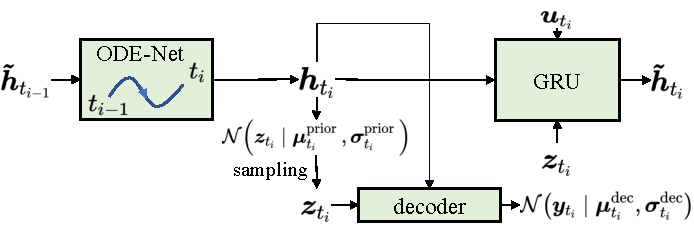
\includegraphics[width=0.9\linewidth]{figures/chapter5/generation.pdf}
%\caption{fig1}
\end{minipage}
\label{fig:generation}
}%
\subfigure[推理模型]{
\begin{minipage}[t]{0.36\linewidth}
\centering
% \hspace{-22pt}
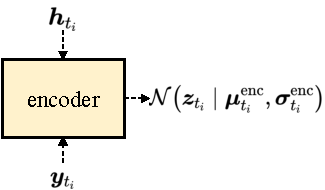
\includegraphics[width=0.9\linewidth]{figures/chapter5/inference.pdf}
%\caption{fig1}
\end{minipage}
\label{fig:5_encoder}
}%
\centering
\caption{ODE-RSSM中的生成过程和推理过程}
\label{fig:5_model_fig}
\end{figure*}
% In this section, we first introduce the components of the ODE-RSSM from two aspects: generative process and inference process, as shown in Fig.~\ref{fig:5_model_fig}.

本节首先介绍ODE-RSSM的生成模型和推理模型,
模型假设隐状态由确定性部分$\hti$和随机部分$\zt$共同组成,即$\boldsymbol{s}_{t_{i}}=[\boldsymbol{z}_{t_{i}},\boldsymbol{h}_{t_{i}}]$。
如图~\ref{fig:5_model_fig}所示。
在生成模型中,模型通过组合门控循环单元(Gate Recurrent Unit, GRU)和ODE网络建模隐状态在非均匀间隔控制输入下的转移过程。
为了训练生成模型参数$\theta$, 本章引入用于近似后验推理的编码器 $q_{\phi}\left(\boldsymbol{z}_{t_i} \mid \boldsymbol{y}_{t_i}, \boldsymbol{h}_{t_i}\right)$对隐变量的真实后验分布进行近似,采用最大化证据下限(Evidence Lower Bound,ELBO)的方式协同训练参数 $\phi$ 和$\theta$。
% 另一方面,本章在训练阶段进一步引入隐空间超调技术\cite{Hafner2019}用于改善模型的多步预测。
% 为了减少引入隐空间超调带来的额外时间开销,本章通过重用临时采样状态的方式显著减少了求解多步KL散度的时间复杂度,有效优化了训练效率。

% 在本章提出的ODE-RSSM模型中,
% 将确定性转移函数$\widetilde{p}_{\theta}(\b h_{i}|\cdot)$定义为一德塔(Delta)分布,由一个确定性的循环神经网络进行建模。
% 随机隐状态$p_{\theta}\left(\b {z}_{t} \mid \b {h}_{t}\right)$和解码网络$p_{\theta}\left(\b {y}_{i} \mid \bold {h}_{i},\b {z}_{i}\right)$的条件分布均为参数化的高斯分布。

% The evolution of the stochastic latent state $\b z_t$ and deterministic hidden state $\b h_t$ represent the transitions in the identified model with the input signal $\b u_t$.  
% Generally, the parameters $\theta$ are learned by jointly introducing approximate posterior encoder $q_{\phi}\left(\boldsymbol{z}_{i} \mid \boldsymbol{y}_{i}, \boldsymbol{h}_{i}\right)$ and maximizing evidence lower bound (ELBO):


% \begin{equation}
% \begin{aligned}
% \widetilde{\mathcal{L}}(\theta, \phi)=& \sum_{t=1}^{N} E_{q_{\phi}\left(\boldsymbol{z}_{t} \mid \boldsymbol{y}_{t}, \boldsymbol{h}_{t}\right)}\left[\log p_{\theta}\left(\boldsymbol{y}_{t} \mid \boldsymbol{z}_{t}\right)\right]-\\
% & \mathrm{KL}\left(q_{\phi}\left(\boldsymbol{z}_{t} \mid \boldsymbol{y}_{t}, \boldsymbol{h}_{t}\right) \| p_{\theta}\left(\boldsymbol{z}_{t} \mid \boldsymbol{h}_{t}\right)\right)
% \end{aligned}
% \label{equ:elbo_single}
% \end{equation}
% With the generative model $p_\theta$ and a sampled latent state inferred from posterior model, the distributions of the latent states and observations in future can be predicted in open loop given sequential inputs.
% 利用后验编码器可以推断隐状态的后验分布,给定从分布中采样的初始隐状态,利用生成模型$p_\theta$,可以在给定序列输入下,对系统隐状态和系统输出值进行开环预测。
% 给定从后验模型推断的隐状态分布中采样的初始隐状态,

% \subsection{Neural Ordinary Differential Equations}
% Neural Ordinary Differential Equations (NODE)~\cite{chen2018neuralode} is a learnable ODE whose derivatives are parameterized by neural networks. 
% The system with specific controlled inputs can be modeled as ODEs by incorporating the inputs $\b u_t$ as a known ODE process~\cite{zhong2019symplectic}:
% \begin{equation}
% \left[
% \begin{aligned}
% \boldsymbol{\dot h}(t)\\
% \boldsymbol{\dot u}(t)
% \end{aligned}
% \right]=
% \left[
% \begin{aligned}
% f_\theta(\boldsymbol{h}(t),\boldsymbol{u}(t),)\\
% \boldsymbol{\dot u}(t)
% \end{aligned}
% \right]
% \end{equation}
% where $\theta$ denotes the parameters in the neural network.
% The solution $\boldsymbol h(t_1)$ at arbitrary time $t_1$ can be solved by using the numerical ODE solver given an initial state $\boldsymbol h(t_0)$:

% %integrating the ODE function with numerical ODE solver:
% \begin{equation}
% \begin{aligned}
%     \boldsymbol h(t_1)&=\text{ODE Solve}(f_\theta,\boldsymbol h(t_0), \boldsymbol u,t_0, t_1)\\
%     &=\boldsymbol h(t_0) + \int_{t_{0}}^{t_{1}} f_\theta(\boldsymbol{h}(t), \boldsymbol u(t), t) d t.
% \end{aligned}
% \end{equation}
% The training of the network parameters $\theta$ is memory-efficient by introducing adjoint sensitivity algorithm\cite{chen2018neuralode}.



% \subsection{连续时间域下含随机隐变量的生成模型}
\subsection{带有随机隐变量的连续时间的生成模型}

% In industrial system controlling, the  $r\left(\boldsymbol{s}(t), \boldsymbol{a}(t)\right)$ is usually a 

% In MPC, we find a policy $\pi$ to maximize the reward integral:
% \begin{equation}
% \pi^*(t) =\arg\max_{\pi}\int_t^{t+T} r(\tau) d\tau\quad \text{s.t. \ dynamic in } \eqref{equ:dynamical}
% \end{equation}

% To model the uncertainty of the dynamical system, we introduce deep state space model with latent variables $\zt$ to identify the evolution of dynamical system.
% ODE-RSSM is a temporal extension of VAE.
% The generative process is a conditional probabilistic model which describes the joint probability distributions of latent states and system outputs under given system inputs.
% With an initial $\b{s}_{t_1}$, the conditional prior of $\st$ is controlled by system inputs:
ODE-RSSM采用带有隐变量的条件概率模型表示序列生成过程,其描述了在给定系统输入条件下隐变量和系统输出的联合概率分布。
给定初始时刻隐变量$\b{s}_{t_1}$, 序列变量$\st$的条件先验分布由系统输入决定:
\begin{equation}
p\left(\boldsymbol{s}_{t_{i}} \mid \boldsymbol{s}_{t_{i-1}}, \boldsymbol{u}_{t_{i-1}}\right)=p\left(\boldsymbol{z}_{t_{i}} \mid \boldsymbol{h}_{t_{i}}\right)*
p\left(\boldsymbol{h}_{t_{i}} \mid \boldsymbol{s}_{t_{i-1}}, \boldsymbol{u}_{t_{i-1}}\right)
\label{equ:prob_latent}
\end{equation}

% The Dirac distribution $p\left(\boldsymbol{h}_{t_{i}} \mid \boldsymbol{z}_{t_{i-1}}, \boldsymbol{u}_{t_{i-1}}\right)$ is determined under the latent state and system inputs in last sampling time step $t_{i-1}$.
% In Eq.~\eqref{equ:prob_latent}, $p\left(\boldsymbol{h}_{t_{i}} \mid \boldsymbol{h}_{t_{i-1}}, \boldsymbol{u}_{t_{i-1}}\right)$ is a Dirac distribution and $\hti$ is deterministic given latent states and system inputs in last sampling time step $t_{i-1}$.
在式~\eqref{equ:prob_latent}中, $p\left(\boldsymbol{h}_{t_{i}} \mid \boldsymbol{s}_{t_{i-1}}, \boldsymbol{u}_{t_{i-1}}\right)$为德尔塔$\delta$分布,在给定$t_{i-1}$时刻的隐变量$\stm$和系统输入$\utm$下,$\hti$是确定的。
% Because the sampling interval $t_i - t_{i-1}$ at different positions $i$ are not uniform in irregular setting, 

本章中不同时刻$t_i$的采样间隔$t_i - t_{i-1}$不是恒等的,
% the common discrete-time sequential models are not applicable to model the evolution of latent states on varying time range. 
一般的离散时间序列模型不适用于建模可变时间间隔下的隐状态演化。
因此,本章受常微分方程网络模型\cite{chen2018neuralode,Rubanova2019}的启发,引入ODE-Net学习确定性隐状态$\hti$在相邻采样时间点之间的演化。

具体地,确定性隐状态$\hti$的转移过程分为两个阶段。
在第一阶段,采用门控循环单元(Gate Recurrent Unit, GRU)建模系统输入$\utm$以及$\ztm$对当前状态$\htm$的瞬时影响,并构建中间变量$\thtm$:
% Concretely, the generative process of $\hti$ consists two stages.
% In the first stage, we employ a GRU network to model the influences from the system input $\ut$ and $\zt$ on the last state $\htm$ and produce an intermediate variable $\thtm$:
\begin{equation}
\thtm  = \text{GRU}(\left [\utm, \ztm\right], \htm)
\label{equ:gru}
\end{equation}
% where $\ct$ denotes the cell state of GRU cell.
下一步,引入参数化ODE-Net $f_\theta$用于建模$\b h_{t}$在时间范围$[t_{i-1},t_{i}]$内对时间$t$的导数,通过求解ODE预测时间点$t_i$处的更新状态$\hti$:
% Next, we introduce a parametric ODE-Net $f_\theta$ to model the CT evolution of $\hti$ and the updated state at next time point can be predicted by solving the ODE:
% $\thti$ represents the predicted deterministic state at $t_i$
\begin{equation}
\begin{aligned}
   \hti&=\text{ODE Solve}(f_\theta, \tilde{\b{h}}_{t_{i-1}}, t_{i-1}, t_i) \\
   &= \tilde{\b{h}}_{t_{i-1}} + \int_{t_{i-1}}^{t_i}f_\theta(\b h_t, \utm, ) \text{d}t
   \label{equ:ode}
\end{aligned}
\end{equation}
% 此处,将系统输入$\utm$作为常微分方程的输入,被定义为分段恒定函数$\b u[t_{i-1},t_i]=\utm$。
积分时间范围内的系统输入被定义为分段恒定函数$\b u[t_{i-1},t_i]=\utm$,将其作为ODE的输入以控制隐状态对时间的导数,进而实现输入输入系统辨识的目的。
在线预测场景下,上述定义方式能够很好地适配控制信号$\ut$是间断采集的情况。
% Common ODE-Nets employ Multilayer Perceptron MLPs to model the derivative functions.
在上述生成过程中,$\htm$表示在获得$\utm$之前,$t_{i-1}$时刻的确定性隐状态的预测结果。
而$\thtm$表示在给定$\ztm$和$\utm$的信息之后更新的隐状态。
$\hti$表示在不给定$t_{i-1}$时刻之后任何信息的情况下,模型自回归预测确定性隐变量在$t_i$时刻的取值。

一般的常微分方程网络采用多层感知机建模导数函数。
本文第三章研究表明,对导数进行积分会导致隐状态范围不断增加且会增加累积误差。因此增量式的ODE网络不适用于长时间序列预测和系统辨识问题。
本章提出一种正交的导数网络定义方法~\cite{jia2019neural}:
\begin{equation}
\frac{d \b h(t)}{dt}=NN_{\theta}(\b h(t))-\frac{\b h(t)}{|\b h(t)|}*\frac{<{NN_{\theta}(\b h(t))},{\b h(t)}>}{|\b h(t)|},
\end{equation}
其中,$NN_{\theta}(\cdot)$是标准的多层感知机,$<\cdot, \cdot>$是向量内积。 
普通的ODE单元、稳定的ODE单元以及本章提出的正交ODE单元之间的区别如图\ref{fig:cells}所示。
\begin{figure}[h]
    \centering
    \subfigure[普通ODE单元]{
    % \begin{minipage}[t]{0.3\linewidth}
    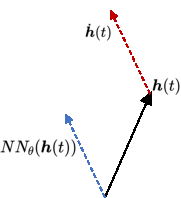
\includegraphics[width=0.3\linewidth]{figures/chapter5/normal.pdf}
    % \end{minipage}
    }
    % \hfill
    \subfigure[稳定ODE单元]{
    % \begin{minipage}[t]{0.3\linewidth}
    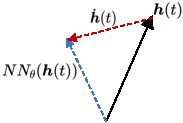
\includegraphics[width=0.3\linewidth]{figures/chapter5/sta.pdf}
    % \end{minipage}
    }
    % \hfill
    \subfigure[正交ODE单元]{
    % \begin{minipage}[t]{0.3\linewidth}
    \includegraphics[width=0.3\linewidth]{figures/chapter5/orth.pdf}
    % \end{minipage}
    }
    % \includegraphics[width=0.3\linewidth]{figs/orth.pdf}
    \caption{三种导数模块定义方法图示}
    \label{fig:cells}
\end{figure}
正交形式保证了导数预测值$\frac{d \b h(t)}{dt}$始终与当前状态$\b h(t)$正交。
因此,从$t_{i-1}$到$t_{i}$的积分过程中,只会改变$\b h(t)$的方向,其范数不变。
$|\b h(t)|$仅由每次GRU网络更新过程决定,且被严格限制在$[-1,1]$。
这种导函数网络结构改进方法能够避免长采样间隔下由于增量式更新导致的隐状态范围过大的问题。
% 一般的

求解常微分方程得到$\hti$后,进而预测$\zt$的先验高斯分布:
% Here, the system input $\utm$ is regarded as a piecewise constant signal, which is not changed until $\ut$ is given.
% After solving the $\hti$ by integrating the derivative determined by the ODE function, the prior Gaussian distribution of $\zt$ is predicted:
\begin{equation}
  p_{\theta}\left(\boldsymbol{z}_{t_{i}} \mid \boldsymbol{h}_{t_{i}}\right) = \mathcal{N}(\zt\mid\boldsymbol{\mu}_{t_i}^{\text {prior }}, \boldsymbol{\sigma}_{t_i}^{\text {prior }})  
  \label{equ:prior_z}
\end{equation}
% where parameters $\boldsymbol{\mu}_{t_i}^{\text {prior }}$ and $\boldsymbol{\sigma}_{t_i}^{\text {prior }}$ are estimated from a Multilayer perceptron(MLP) whose input is the deterministic latent states $\hti$.
其中,采用多层感知机模型估计分布参数$\boldsymbol{\mu}_{t_i}^{\text {prior }}$ 和 $\boldsymbol{\sigma}_{t_i}^{\text {prior }}$,模型输入为确定性的隐状态 $\hti$。
% In the generative process, $\hti$ represents the predicted latent state at time $t_i$ before perceiving the information brought from $\ut$.
% The state $\thti$ denotes the updated state after incorporating the information from $\zt$ and $\ut$.

% In order to predict the distribution of the system outputs , a decoder module is introduced to determine the Gaussian distribution of system outputs $\yt$ under a specific latent states:
为了预测系统输出分布,进一步引入解码器模块预测系统输出$\yt$在给定隐状态$\st$下的高斯分布:
\begin{equation}
    p\left(\boldsymbol{y}_{t_{i}} \mid \boldsymbol{h}_{t_{i}}, \zt\right) = \mathcal{N}(\yt \mid\boldsymbol{\mu}_{t_i}^{\text {dec }}, \boldsymbol{\sigma}_{t_i}^{\text {dec }})
    \label{equ:output_layer}
\end{equation}
% where the distribution parameters $\boldsymbol{\mu}_{t_i}^{\text {dec}}, \boldsymbol{\sigma}_{t_i}^{\text {dec}}$ depend on both deterministic and stochastic latent states.
分布参数$\boldsymbol{\mu}_{t_i}^{\text {dec}}, \boldsymbol{\sigma}_{t_i}^{\text {dec}}$由确定性隐状态和随机隐状态共同决定。
在给定序列系统输入下,通过对序列隐状态分布进行反复预测与采样,模型可以开环地预测序列隐变量并预测系统输出。

% Under given sequential system inputs, the sequential latent states can be predicted in open loop by repeatedly sampling the states $\st$ from the predicted distribution of latent states.
% We can further predict the system outputs based on the decoder module and the sampled latent states.
% 我们可以进一步预测系统输出基于解码器模块和采样的潜伏状态。
% With the sampled latent states, system outputs are predicted directly based on decoder module.
% The 
% With a trained generative model and given sequential system inputs, we can predict the evolution of latent states and the outputs by sampling the variables $\b{z}, \b{h}$ and system outputs $\b{y}$ recurrently.

% We define the equations \eqref{equ:ode}, \eqref{equ:gru} and decoder as generative model.
% \subsection{Parallel single-step generative process with batched non-uniform sampling intervals}
\subsection{隐变量推理与训练}
% \label{sec:inference_training}
% 基于高效隐空间超调的多步预测性能改善
% In order to train the parameters $\theta$ in the generative model, a regular way is to maximize the log likelihood of system outputs $\mathcal{L}=\sum_{i=1}^N\log p_{\theta}\left( \yt \mid  \b u_{<t_i}  \right)$.
为了训练生成模型中的参数$\theta$,常规方法是最大化系统输出的对数似然$\mathcal{L}=\sum_{i=1}^N\log p_{\theta}\left( \yt \mid  \b u_{<t_i}  \right)$。
% Because it is intractable to solve the exact posterior $\b{s}_{t_1:t_N}$, we cannot estimate the exact $\mathcal{L}$ by averaging the log likelihood over the probability of all possible values.
因为直接计算隐变量$\b{s}_{t_1:t_N}$的精确后验分布是极其困难的,因此无法采用对隐变量概率分布进行积分的方式估计精确的对数似然$\mathcal{L}$。
% Because it is intractable to solve true posterior distribution of $\b{s}_{t_1:t_N}$ directly with the generative model. 
% Therefore, we adopt a tractable way to both learning and inference by introducing an variational distribution $q_\phi$ to infer the approximate posterior distribution of the stochastic latent state:
本章引入变分分布$q_\phi$近似随机隐变量的后验分布,进而辅助生成模型的学习。
 % $\{\ut\}_{i=1}^{N}$ and $\{\yt\}_{i=1}^{N}$
\begin{equation}
\begin{aligned}
 q_{\phi}(\b z_{t_1:t_N}\mid\b y_{t_1:t_N},\b u_{t_1:t_N}) &= \prod_{i=1}^{N} q_{\phi}(\b z_{t_i}\mid \b{h}_{t_i},\yt)\\
 &= \prod_{i=1}^{N} \mathcal{N}(\zt\mid\boldsymbol{\mu}_{t_i}^{\text {enc }}, \boldsymbol{\sigma}_{t_i}^{\text {enc }})  
 \label{equ:posterior_z}
\end{aligned}
\end{equation}
% As shown in Fig.~\ref{fig:5_encoder}, the variational distribution $q_\phi(\zt|\cdot)$ is a Gaussian distribution whose parameters $\boldsymbol{\mu}_{t_i}^{\text {enc }}$ and $\boldsymbol{\sigma}_{t_i}^{\text {enc }}$ are estimated from the encoder module, built as a MLP.
如图\ref{fig:5_model_fig}\subref{fig:5_encoder}所示,变分分布$q_\phi(\zt|\cdot)$为高斯分布,其分布参数$\boldsymbol{\mu}_{t_i}^{\text {enc }}$ 和 $\boldsymbol{\sigma}_{t_i}^{\text {enc }}$由基于MLP网络构建的编码器模块进行估计。
% Where both $\boldsymbol{\mu}_{t_i}^{\text {enc }}$ and $\boldsymbol{\sigma}_{t_i}^{\text {enc }}$ are inferred from an encoder model, as shown 
% Because solving $\hti$ requires the previous stochastic latent states $\b z_{<t_i}$, the generative process and inference process are alternating for inferring the sequential posterior $q_{\phi}(\b z_{t_1:t_N}\mid\b y_{t_1:t_N},\b u_{t_1:t_N})$.
因为求解 $\hti$ 需要之前的随机隐状态 $\b z_{<t_i}$, 在推理序列后验$q_{\phi}(\b z_{t_1:t_N}\mid\b y_{t_1:t_N},\b u_{t_1:t_N})$时,生成过程和推理过程是被交互调用,不断采样出新的$\zt$并预测$\hti$。
% the generative process and inference process are alternating for inferring the sequential posterior $q_{\phi}(\b z_{t_1:t_N}\mid\b y_{t_1:t_N},\b u_{t_1:t_N})$.

% during inferring the posterior distributions of $\b z$.
% because the previous stochastic latent states $\b z_{<t_i}$ are required for solving $\hti$, the generative and inference processes are alternating during estimating the posterior distributions of $\b z$.

% The ODE-RSSM model is trained by maximizing the evidence lower bound(ELBO) of the observed system outputs:  
利用后验推理分布,可以通过最大化系统观测证据下界的方式训练ODE-RSSM模型:

\begin{equation}
\begin{aligned} 
\ln p\left(\boldsymbol{y}_{t_{1}: t_{N}}\right)&=\ln \int \prod_{i=1}^{N} p\left(\boldsymbol{s}_{t_{i}} \mid \boldsymbol{s}_{t_{i-1}},\boldsymbol{u}_{t_{i-1}} \right) p\left(\boldsymbol{y}_{t_{i}} \mid \boldsymbol{s}_{t_{i}}\right) d \boldsymbol{s}_{t_{1}: t_{N}} \\ 
 &\geq\sum_{i=1}^{N}\left(\mathrm{E}_{q(\boldsymbol{s}_{t_{i}})}\left[\ln p\left(\boldsymbol{y}_{t_{i}} \mid \boldsymbol{s}_{t_{i}}\right)\right]\right.\\
% &\hspace{-10ex}\quad
&-\left.\mathrm{E}_{q(\boldsymbol{s}_{t_{i}})}\left[\operatorname{KL}\left[q(\boldsymbol{s}_{t_{i}}) \| p\left(\boldsymbol{s}_{t_{i}} \mid \boldsymbol{s}_{t_{i-1}},\boldsymbol{u}_{t_{i-1}}\right)\right]\right]\right)
% \\[-5pt]
% &\ \tiny{{q(\boldsymbol{s}_{t_{i}})}}
\end{aligned}
\label{equ:loss_single}
\end{equation}
% where $q(\boldsymbol{s}_{t_{i}})$ is the abbreviation of $q_\phi\left(\boldsymbol{s}_{t_{i}} \mid \boldsymbol{y}_{\leq t_i},\boldsymbol{u}_{<t_{i}} \right)$.
为了表述方便,此处将 $q_\phi\left(\boldsymbol{s}_{t_{i}} \mid \boldsymbol{y}_{\leq t_i},\boldsymbol{u}_{<t_{i}} \right)$ 简记为$q(\boldsymbol{s}_{t_{i}})$。

% In addition to approximating the posterior distribution for estimating the log likelihood in training phase, the inference model is also capable of representing the system state as a temporal encoder model.
对于推理模型,除了可以用于近似隐变量的后验分布以估计证据下限外,推理模型还可作为序列编码模型用于对系统状态进行编码。
% As an recurrent encoder-decoder framework, the ODE-RSSM carries an encoder for inference and and generative model for prediction.
作为支持状态循环更新的编码器-解码器框架,ODE-RSSM可以灵活地采用推理模型进行隐变量推断并采用生成模型进行在线预测。
在一些具有流式数据的在线任务中,两个模块可能需要被迭代调用。
例如,在模型预测控制问题中,利用推理模型可以对给定的历史输入输出数据进行编码以得到隐状态的后验分布并采样,利用生成模型可以对任意给定控制输入下的系统输出进行预测,进而辅助系统控制。
% Both parts are iteratively called in some tasks with online streaming data.
% For example, in model prediction control, the inference model is utilized to infer the latent states given historical monitored system outputs and the generative model predicts the system outputs under optimized control inputs.
% With the inferred state, we can predict the system outputs under optimized control inputs via generative model.

% The ODE-RSSM model is trained by maximizing the 




% The output distribution is also defined as a normal distribution, $p_{\theta}\left(\b{y}_{t_i} \mid \b{z}_{t_i}\right)=\mathcal{N}\left(\b{y}_{t_i} \mid \boldsymbol{\mu}_{t_i}^{\mathrm{dec}}, \boldsymbol{\sigma}_{t_i}^{\mathrm{dec}}\right)$.


% Concretely, the conditional distributions of both latent variables $\zt$ and $\yt$ can be factorized as follows:
% \begin{alined}
% p_{\theta}() = 
% \end{alined}

% \subsection{Efficient latent overshooting for improving long-term prediction}
\section{基于高效隐空间超调的多步预测性能改善}
\label{sec:5_overshooting}
% In multi-step planning, the model is required to make multi-step predictions~\cite{Hafner2019} according to the inputs sequence.
在基于模型的序贯决策问题中,模型需要根据给定的控制输入序列进行多步预测~\cite{Hafner2019}。
% In this case, the generative model is iteratively applied, feeding through the latent states sampled from the previous predicted prior distribution as its new inputs.
对于ODE-RSSM,需要重复地调用生成模型进行隐变量的单步预测,并从预测分布中采样得到隐状态,将其作为下一步预测的输入。
% 这种情况下,
% In multiple-step simulation, 
% However, in the loss function defined in Eq.\eqref{equ:loss_single}, the KL divergence is only measured between the approximate posterior distribution and the single-step predicted distribution.
然而,对于式\eqref{equ:loss_single}定义的损失函数,其KL散度项仅度量了近似后验分布和单步预测分布之间的差异。
因此,在模型训练时,反向传播的梯度流只对生成模型的单步预测过程进行了优化。
另外,在训练过程中,生成模型预测时的隐变量输入始终来自于近似后验分布的采样。
而多步预测时,其隐变量输入大多数情况下来源于生成模型给出的预测分布。
% The gradient flow in back propagation merely optimizes the generative model in one-step prediction.
% The distinction between the posterior and prior breaks the train-test i.i.d assumption on the inputs of generative model, which may lead to poor accuracy in multi-step predictions\cite{venkatraman2015improving}. 
近似后验分布和预测先验分布之间的差异打破了生成模型的隐变量输入在训练集和测试集上的同分布假设,这会导致多步预测的准确性较差\cite{venkatraman2015improving}。
% This drawback is more serious in the complicated systems with long-time delay and partially observed space.
对于观测空间不完备的不确定性复杂系统,这一问题将更加明显。
% 这一缺陷在时滞较长、观测空间不全的复杂系统中更为严重。
% Because 
% For complicated systems with long-time delay and partially observed space, training the sequential model with single-step loss may lead to poor accuracy in multi-step predictions\cite{venkatraman2015improving}. 
% of model which is only trained to make perfect one-step predictions.
% Therefore, we introduce the latent overshooting technique~\cite{Hafner2019} in ODE-RSSM to improve multi-step predictions in generative process.
因此,本章在ODE-RSSM的训练过程中引入了隐空间超调技术~\cite{Hafner2019}用于改善生成过程中的多步预测性能。

% Concretely, the multi-step prediction of latent states with a fixed distance $d$ is defined as:
具体地,对于长度为$d$的多步隐状态预测过程可以表示为:
\begin{equation}
\begin{aligned}
p\left(\boldsymbol{s}_{t_i} \mid \boldsymbol{s}_{t_{i-d}}\right) & \triangleq \int \prod_{\tau=i-d+1}^{i} p\left(\boldsymbol{s}_{t_\tau} \mid \boldsymbol{s}_{t_{\tau-1}},\boldsymbol{u}_{t_{\tau-1}}\right) \mathrm{d} \boldsymbol{s}_{t_{i-d+1}: t_{i-1}} \\
&=\mathrm{E}_{p\left(\boldsymbol{s}_{t_{i-1}} \mid \boldsymbol{s}_{t_{i-d}}\right)}\left[p\left(\boldsymbol{s}_{t_i} \mid \boldsymbol{s}_{t_{i-1}}\right)\right]
\end{aligned}
\label{equ:multistep}
\end{equation}
% As integrating the probability density of intermediate latent states is intractable, 
% Because it is intractable to solve the analysis multi-step prediction distribution by integrating the probability density of all intermediate latent states, 
% 由于对所有中间隐变量的概率密度进行积分求解分析多步预测分布是很困难的,
% 由于通过对所有中间隐变量的概率分布进行积分的方式求解多步预测分布是极其困难的。
想要精确地求解$\boldsymbol{s}_{t_{i-d}} $下$\boldsymbol{s}_{t_{i}}$的多步预测分布,常规方法是对所有中间隐变量的概率分布进行积分,但在实际应用中这是极为困难的。
% Because it is intractable to integrate the probability density of all intermediate latent states and solve the analytical joint multi-step prediction distribution,
% we generally employ the ancestral sampling and reparameterization trick to repeatedly sample the intermediate states from one-step predicted distribution for multi-step prediction.
对于多步预测,可以采用多次祖先采样(Ancestral sampling)和重参数化技巧(Reparameterization Trick)不断地对单步预测分布中的中间状态进行采样。最终$\boldsymbol{s}_{t_{i}}$的采样分布将服从多步预测的理论分布。

% On the basis of the $d$-steps prior distribution defined by Eq.\eqref{equ:multistep}, we next derive a new ELBO on multi-step prediction which is a lower bound on the one-step prediction ELBO in \eqref{equ:elbo_single} and the original log likelihood of system outputs.
% On the basis of the $d$-steps prior distribution defined by Eq.\eqref{equ:multistep}, we next derive a new ELBO on the multi-step prediction:
基于式\eqref{equ:multistep}定义的$d$-步预测先验分布,进而可以推导出定义在多步预测先验分布上的ELBO:
% On the basis of the $d$-steps prior distribution defined by Eq.\eqref{equ:multistep}, a new ELBO on multi-step prediction which is a lower bound on the one-step prediction ELBO in \eqref{equ:elbo_single} and the original log likelihood of system outputs.
% $q\left(\boldsymbol{s}_{t_{i}} \mid \boldsymbol{y}_{\leq t_i},\boldsymbol{u}_{<t_{i}} \right)$
% $q\left(\boldsymbol{s}_{t_{i}}\right)$
\begin{equation}
\begin{aligned} \ln p_d\left(\boldsymbol{y}_{t_{1}: t_{N}}\right)&=\ln \int \prod_{i=1}^{N} p\left(\boldsymbol{s}_{t_{i}} \mid \boldsymbol{s}_{t_{i-d}} \right) p\left(\boldsymbol{y}_{t_{i}} \mid \boldsymbol{s}_{t_{i}}\right) d \boldsymbol{z}_{t_{1}: t_{N}} \\ 
& \geq\sum_{i=1}^{N}\left(\mathrm{E}_{q\left(\boldsymbol{s}_{t_{i}}\right)}\left[\ln p\left(\boldsymbol{y}_{t_{i}} \mid \boldsymbol{s}_{t_{i}}\right)\right]\right.\\
&\hspace{-1ex}\quad\begin{aligned}
-&\left.\mathrm{E}\left[\operatorname{KL}\left[q\left(\boldsymbol{s}_{t_{i}}\right)\| p\left(\boldsymbol{s}_{t_{i}} \mid \boldsymbol{s}_{t_{i-1}},\boldsymbol{u}_{t_{i-1}}\right)\right]\right]\right)\\[-5pt]
&\ \tiny{p\left(\boldsymbol{s}_{t_{i-1}} \mid \boldsymbol{s}_{t_{i-d}}\right){q\left(\boldsymbol{s}_{t_{i-d}}\right)}}
\end{aligned}
\end{aligned}
\label{equ:loss_multi}
\end{equation}
% It can be proved that $\ln p_d\left(\boldsymbol{y}_{t_{1}: t_{N}}\right)$ is a lower bound of the one-step prediction ELBO in \eqref{equ:elbo_single} and the original log likelihood of system outputs.
% According to the proof in ~\cite{Hafner2019}, $\ln p_d\left(\boldsymbol{y}_{t_{1}: t_{N}}\right)$ is a lower bound of the one-step prediction ELBO in \eqref{equ:elbo_single} and the original log likelihood of system outputs.

由前人研究~\cite{Hafner2019}给出的证明, $\ln p_d\left(\boldsymbol{y}_{t_{1}: t_{N}}\right)$ 是式\eqref{equ:loss_single}中单步预测ELBO的下界,自然也是原始系统输出对数似然的下界。最大化$\ln p_d\left(\boldsymbol{y}_{t_{1}: t_{N}}\right)$能够起到增大输出对数似然的目的。
% Given a hyper-parameter $D$, we average the variational bound of all distances $1\leq d\leq D$ to improve multi-step prediction for all possible distances, 
给定超参数$D$,可以对多种可能的预测距离$1\leq d \leq D$的变分下界求平均,以改进不同距离下的多步预测精度:
\begin{equation}
\begin{aligned}
    \text{ELBO-D}&=\frac{1}{D}\sum_{d=1}^{D}\ln p_d\left(\boldsymbol{y}_{t_{1}: t_{N}}\right) \\
     \geq\mathrm{E}_{q(\b s_{t_1:t_N})}&\left[\ln p\left(\b y_{t_1:t_N} \mid \b s_{t_1:t_N}\right)\right]-\frac{1}{D}*\text{KL-D}\
    %  &-\frac{1}{D}*\text{KL-D}
\end{aligned}
\end{equation}
其中
\begin{equation}
\begin{aligned}
\text{KL-D}=\sum_{d=1}^{D}\sum_{i=1}^{N}\mathrm{E}&\left[\operatorname{KL}\left[q\left(\boldsymbol{s}_{t_{i}} \right) \| p\left(\boldsymbol{s}_{t_{i}} \mid \boldsymbol{s}_{t_{i-1}}\right)\right]\right]\\[-15pt]
&{p\left(\boldsymbol{s}_{t_{i-1}} \mid \boldsymbol{s}_{t_{i-d}}\right){q\left(\boldsymbol{s}_{t_{i-d}} \right)}}
\end{aligned}
\label{equ:kld}
\end{equation}
% For simplicity, we omit the $\b u$ and $\b y$ in KL term here.
为简化表述,此处省略了KL散度项中的$\b u$和$\b y$。

% Training the temporal VAE models with multi-step ELBO improves the long-term open loop prediction indeed~\cite{Hafner2019}.
利用多步证据下界训练时序变分自编码机模型能够在一定程度上改善模型的长期开环预测精度~\cite{Hafner2019}。
然而,依照公式\eqref{equ:kld}直接估计KL-D的时间复杂度为$\mathcal{O}(N*D^2)$,除了对于序列不同位置的计算循环$1\leq d \leq D$可以并行化处理,还包括对于最大距离$D$的外循环$1\leq d \leq D$ ,以及式\eqref{equ:multistep}所示的多步预测采样$p\left(\boldsymbol{s}_{t_{i-1}} \mid \boldsymbol{s}_{t_{i-d}}\right)$($\mathcal{O}(d)$)。
% However, the time complexity of estimating KL-D is $\mathcal{O}(N*D^2)$ which includes the external loop $1\leq d \leq D$ for each distance($\mathcal{O}(D)$) and the multi-step sampling $p\left(\boldsymbol{s}_{t_{i-1}} \mid \boldsymbol{s}_{t_{i-d}}\right)$($\mathcal{O}(d)$), as shown in Equ.\eqref{equ:multistep}.
% However, if we estimate the KL-D 
% However, for training ODE-RSSM, estimating KL-D directly is time-consuming.
% However, time-consuming in traning ODE-RSSM
% The time complexity of estimating KL-D directly is $\mathcal{O}(N*D^2)$, 
% \begin{itemize}
%     \item The external loop $1\leq d \leq D$ for each distance:  $\mathcal{O}(D)$
%     \item The internal loop $1\leq i\leq N$ for each position: $\mathcal{O}(N)$
%     \item The multi-step sampling $p\left(\boldsymbol{s}_{t_{i-1}} \mid \boldsymbol{s}_{t_{i-d}}\right)$ as shown in Equ.\eqref{equ:multistep}: $\mathcal{O}(d)$
% \end{itemize}
% In this paper, we provide a optimization to accelerate the estimation of KL-D by merging the external loop and multi-step sampling and making the internal loop parallelizable.
% In this paper, we provide a optimization to accelerate the estimation of KL-D by merging the external loop and multi-step sampling/
% 本章中,
本章提出了一种加速估计KL-D的优化方法,该方法能够合并外循环和多步采样过程的计算复杂度,使估计KL-D的时间复杂度变为$\mathcal{O}(N*D)$。
% \subsubsection{Reusing sampled latent states for avoiding multi-step prediction}
% For differet distance $s$, with a fixed $i-d$ are redundant
% As shown in Eq.\eqref{equ:multistep}, the sampling operations for different distance $d$ are redundant with a fixed $i-d$.
通过分析式\eqref{equ:multistep}可以得知,对于不同的$i,d$,在$i-d$相同的情况下,不管预测距离$d$如何变化,对于$i-d + 1 \leq \tau \leq i-1$下的单步预测过程 $p\left(\boldsymbol{s}_{t_\tau} \mid \boldsymbol{s}_{t_{\tau-1}}\right)$ 存在于所有的多步预测 $p\left(\boldsymbol{s}_{t_{i-1}} \mid \boldsymbol{s}_{t_{i-d}}\right)$中。
% First, as shown in Eq.\eqref{equ:multistep}, the one-step sampling $p\left(\boldsymbol{s}_{t_\tau} \mid \boldsymbol{s}_{t_{\tau-1}}\right)$ with $i-d + 1 \leq \tau \leq i-1$ exists in all of the multi-step sampling $p\left(\boldsymbol{s}_{t_{i-1}} \mid \boldsymbol{s}_{t_{i-d}}\right)$ when $i-d$ is fixed. 
% Therefore, we could reuse the intermediate sampled states $\b{s}_{t_{i-d}:t_{i-1}}$ for all distances $d$ and obtain an unbiased estimation of KL divergence.
因此,对于超调距离$d$不同但后验推理位置$i-d$相同的多步预测,可以共用中间的采样状态$\b{s}_{t_{i-d}:t_{i-1}}$,并得到KL散度的无偏估计。

% Therefore, with an ident beginning position $i-d$ where the approximate posterior distribution is sampled, we could reuse the intermediate sampled states $\b{s}_{t_{i-d}:t_{i-1}}$ for different $d$ to obtain unbiased samples efficiently.

% In details, we rewrite the $\text{KL-D}$ as:
具体地,将KL-D的计算公式重写为:
\begin{equation}
\begin{aligned}
\text{KL-D}=&\sum_{i=1}^{N}\sum_{d=1}^{D}\mathrm{E}\left[\operatorname{KL}\left[q\left(\boldsymbol{s}_{t_{i+d}} \right) \| p\left(\boldsymbol{s}_{t_{i+d}} \mid \boldsymbol{s}_{t_{i+d-1}}\right)\right]\right]\\[-15pt]
&\hspace{40pt}p\left(\boldsymbol{s}_{t_{i+d-1}} \mid\boldsymbol{s}_{t_{i}}\right){q\left(\boldsymbol{s}_{t_{i}} \right)}\\
=&\sum_{i=1}^{N}\mathrm{E}_{\hat{\b{s}}_{t_i}\sim q(\b{s}_{t_{i}})}\mathrm{E}_{p(\b{\hat{s}}_{t_{i+1}:t_{i+D-1}}\mid \hat{\b{s}}_{t_i})}\sum_{d=1}^{D}\operatorname{KL}(i+d)\\
\end{aligned}
\label{equ:reuse}
\end{equation}
% where $\operatorname{KL}(i+d)$ is the abbreviation of $\operatorname{KL}\left[q\left(\boldsymbol{s}_{t_{i+d}} \right) \| p\left(\boldsymbol{s}_{t_{i+d}} \mid \boldsymbol{\hat s}_{t_{i+d-1}}\right)\right]$.
其中 $\operatorname{KL}(i+d)$ 为$\operatorname{KL}\left[q\left(\boldsymbol{s}_{t_{i+d}} \right) \| p\left(\boldsymbol{s}_{t_{i+d}} \mid \boldsymbol{\hat s}_{t_{i+d-1}}\right)\right]$的缩写。
% $\b{\hat{s}}_{t_{i}}$ is sampled from the posterior distribution and $\b{\hat{s}}_{t_{i+1}:t_{i+D-1}}$ are sampled based on ancestral sampling, iteratively sampling the states from one-step predicted distribution and feeding the samples as inputs for predicting a new one .
$\b{\hat{s}}_{t_{i}}$是从后验推理分布中采样的初始状态,
% $\b{\hat{s}}_{t_{i+1}:t_{i+D-1}}$ 
% are sampled based on ancestral sampling, iteratively sampling the states from one-step predicted distribution and feeding the samples as inputs for predicting a new one .
$\b{\hat{s}}_{t_{i+1}:t_{i+D-1}}$为采用祖先采样法逐步预测采样得到的序列隐状态。
改进后的采样方法能够获得KL-D的无偏估计,且其时间复杂度仅为$\mathcal{O}(N\times D)$。
% where the first prediction distribution $p\left(\boldsymbol{\hat{s}}_{t_{i}} \mid\boldsymbol{\hat{s}}_{t_{i-1}}\right)$ with $d=1$ is replaced with the inferred posterior distribution $q(\b{s_{t_i}})$.
% and $p\left(\boldsymbol{\hat{s}}_{t_{i+d-1}} \mid\boldsymbol{\hat{s}}_{t_{i+d-2}}\right)$ is the single step prediction distribution.
% where the fir state $\hat{\b{s}}_{t_i}$ with $d=0$ is sampled from the inferred posterior distribution  $q(\b{s_{t_i}})$ and $p\left(\boldsymbol{\hat{s}}_{t_{i+d-1}} \mid\boldsymbol{\hat{s}}_{t_{i+d-2}}\right)$ is the single step prediction distribution.
% $\hat{\b{s}}_{t_i}=\st$ and $\hat{\b{s}}_{t_{i+d}} \sim p\left(\boldsymbol{s}_{t_{i+d}} \mid \boldsymbol{\hat s}_{t_{i+d-1}}\right)$.
% The multi-step sampling is pruned. 
% The illustration of sampling and calculating KL divergence is shown in Fig.\ref{fig:overshooting}.
隐状态采样和计算KL散度的过程如图\ref{fig:overshooting}所示。
% The illustration is shown in Figure.~\ref{fig:overshooting}.
\begin{figure}[ht]
    \centering
    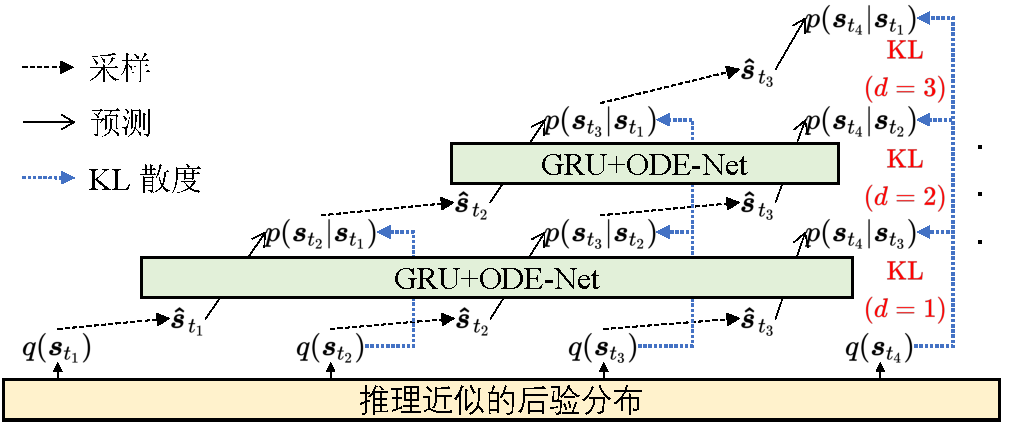
\includegraphics[width=0.9\linewidth]{figures/chapter5/overshooting.pdf}
    % \caption{Latent overshooting based on ancestral Sampling}
    \caption{基于祖先采样的高效隐空间超调}
    \label{fig:overshooting}
\end{figure}
% With the proposed technique in \ref{sec:parallel_ode_solve} for solving the batched ODEs in parallelizable, 
% By introducing the batched ODEs solver stated in \ref{sec:parallel_ode_solve} for parallelizing the loop $1\leq i\leq N$ in \eqref{equ:reuse}, the practical time consumption for estimating KL-D grows linearly as the maximal overshooting length $D$ when the memory of GPUs is enough.
% By parallelizing the loop $1\leq i\leq N$ in Eq.\eqref{equ:reuse} based on the batched ODEs solver stated in \ref{sec:parallel_ode_solve}, the practical time consumption for estimating KL-D grows linearly as the maximal overshooting length $D$ when the memory of GPUs is enough.

本章提出的高效隐空间超调技术能够在仅增加较小训练开销的代价下,显著提升模型的多步预测能力,且该方法对于其他深度状态空间模型的训练同样具有适用性。
% The complete algorithm for solving KL-D is summarized in Alg.~\ref{alg:parallel_overshooting}.

% \subsubsection{Summary}
% To sum up the two optimizations, the complexity of estimating unbiased KL-D is optimized to $\mathcal{O}(ND)$ by reusing the sampled latent states Equ.\eqref{equ:reuse} and the main loop with complexity $\mathcal{O}(N)$ is parallelizable.
% In practice, the actual time consumption for estimating KL-D grows linearly as the maximal overshooting length $D$ the when the memory of GPUs is enough.

% where
% \begin{equation}
% \begin{aligned}
% &\text{d}\b{T}=\b{T}_{i+1}-\b{T}_i\\
% &\b{k}_{0}=f_\theta(\b{\tilde H}_{\b{T}_{i}}  ) \\
% &\b{k}_{1}=f_\theta\left(\b{\tilde H}_{\b{T}_{i}}+\frac{1}{2} \text{d}\b{T} \b{k}_{0}  \right) \\
% &\b{k}_{2}=f_\theta\left(\b{\tilde H}_{\b{T}_{i}}+\frac{1}{2} \text{d}\b{T} \b{k}_{1}  \right) \\
% &\b{k}_{3}=f_\theta\left(\b{\tilde H}_{\b{T}_{i}}+\text{d}\b{T} \b{k}_{2} \right)
% \end{aligned}
% \label{equ:RK}
% \end{equation}

% In Equ\eqref{equ:RK}, the operations of dot product and estimating derivative via ODE-Net $f_\theta$ are both parallelizable.
% The complete algorithm \mathbf{Latent overshooting based on parallel ancestor sampling} is shown in Alg.\ref{alg:parallel_overshooting}.
%  To improve the long-term prediction, we introduce latent overshooting method in ODE-RSSM and provide an parallel acceleration technique to reduce the time complexity of estimating KL divergence.
% To improve long-term predictions of generative process, we introduce a efficient latent overshooting method in training stage.
% By substituting fixed-order RK solver for adaptive ode-solver when solving batched hidden states with misaligned time steps, 
% the method accomplishes parallel prediction of hidden states for batched irregular sampled sequences and reduces the time complexity of estimating KL divergence as $\mathcal{O}(D)$ 
% \begin{algorithm}
% \caption{2333}\label{233}
% \begin{algorithmic}[1]
% \Statex \mathbf{Input:} 233
% \Statex \mathbf{Output:} 23333
% \State 2233
% \end{algorithmic}
% \end{algorithm}

% \begin{algorithm}
% % \caption{Latent overshooting based on parallel ancestor sampling}
% \caption{Batched ancestor sampling for estimating KL-D}
% \begin{algorithmic}[1]
% \Statex \mathbf{Input: } The generative networks (an ODE-Net $f_\theta$ and a GRU), the encoder for posterior inferring, sequential inputs $\b u_{t_1:t_N}$ and sequential outputs $\b y_{t_1:t_N}$
% % \Statex \mathbf{Output:} $\text{KL-D}(q_{\phi}(\b z_{t_1:t_N})||p_{\theta}(\b z_{t_1:t_N}|\b u_{t_1:t_N}))$ 
% \Statex \mathbf{Output:} $\text{KL-D}$ 
% % \State Solving $\b{{h}}_{t_1:t_N}$ according to \eqref{equ:gru} and \eqref{equ:ode}, 
% % \State inferring the posterior distribution $q_{\phi}$ and sampling $ \b{z}_{t_1:t_N}\sim q_{\phi}(\b z_{t_1:t_N}|\b h_{t_1:t_N}, \b y_{t_1:t_N})$. 
% % \State Sampling $\b{z}_{t_1:t_N}$ and $\b{{h}}_{t_1:t_N}$ from the approximate posterior distribution $q_{\phi}(\b z_{t_1:t_N}|\b h_{t_1:t_N}, \b y_{t_1:t_N})$ and the generative process \eqref{equ:gru} and \eqref{equ:ode}, . 
% \State Iteratively sampling $\b{z}_{t_1:t_N}$, $\b{{h}}_{t_1:t_N}$ and inferring $q_{\phi}(\b z_{t_1:t_N}|\b h_{t_1:t_N}, \b y_{t_1:t_N})$ according to Eq.~\eqref{equ:gru}, \eqref{equ:ode}, and \eqref{equ:posterior_z}.
% \State Initializing $\hat{\b{z}}_{t_1:t_N}=\b{z}_{t_1:t_N}$, $\hat{\b{h}}_{t_1:t_N}=\b{h}_{t_1:t_N}$
% % \State Sampling $ \b{\hat z}_{t_1:t_N}\sim q_{\phi}(\b z_{t_1:t_N}|\b u_{t_1:t_N},\b y_{t_1:t_N})$ and solving $\b{\tilde{H}}_{t_1:t_N}$ according to posterior distribution $q_{\phi}$, \eqref{equ:gru} and \eqref{equ:ode}.;
% \For{$d:=1 \text{ to } D$}
% % \Begin
% \State GRU updating for deterministic latent states: $\tilde{\b{h}}_{t_d:t_N}=\text{GRU}(\left [\b{u}_{t_d:t_N}, \hat{\b{z}}_{t_d:t_N}\right], \b{{\hat h}}_{t_d:t_N})$
% % $\left[\b{h}_{t_d:t_N},\b{c}_{t_{i+1}:t_{N+1}}\right]=\text{GRU}(\left [\b{u}_{t_d:t_N}, \b{z}_{t_d:t_N}\right], \left[\b{\tilde{h}}_{t_d:t_N},\b{c}_{t_d:t_N}\right])$
% \State Solving $\b{{\hat h}}_{t_{d+1}:t_{N}}$ according to \eqref{equ:parallel_solver} with $g_{\theta}=f_{\theta}(\boldsymbol{R}(t)) \circ\left(t_{d+1}:t_N-t_d:t_{N-1}\right)$ and $\boldsymbol{R}(0)=\tilde{\b{h}}_{t_d:t_{N-1}}$.
% \State $\text{KL}^d= \text{KL}\left[p(\b{z}_{t_{d+1}:t_{N}}\mid \b{{h}}_{t_{d+1}:t_{N}})||q(\b{z}_{t_{d+1}:t_N})\right]$
% % \End
% \EndFor
% \State Return $\text{KL-D} = \sum_{i=1}^{D}\text{KL}^d$ 
% \end{algorithmic}
% \label{alg:parallel_overshooting}
% \end{algorithm}

% \begin{algorithm*}[]
% \caption{ 基于DFA-ODEnets的编码器-解码器训练过程 }
% \label{alg:training}
% \begin{algorithmic}[1]
% \For{每一个训练轮次}
% \For{$k$ steps}
% \State  在训练集$S$中随机抽样一批序列 $\{\boldsymbol{Y}_{1:I+L}, {\boldsymbol {X}}_{1:I+L}\}$.
% \State \text{//}\textit{为了加快训练速度,下面的步骤是并行执行的.}
% \State 给训练数据的各阶段打标签: $s_{t_1:t_{I+L}}$
% \State 使用样条插值来处理离散序列${\boldsymbol {X}}_{1:I+L}$, $\boldsymbol{Y}_{1:I+L}$,生成$[t_1, t_{I+L}]$的连续序列 $\boldsymbol X(t)$ 和$[t_1, t_{I}]$的连续序列 $\boldsymbol Y(t)$。
% \State 编码阶段: DFA-ODEnet编码器根据条件范围下的系统输入和输出序列估计初始状态 $\boldsymbol{S}\left(t_{I}\right)$,\eqref{equa:initial_state}。
% \State 预测阶段: DFA-ODEnet解码器根据预测范围下的系统输入 $[t_I, t_{I+L}]$预测离散时间点$\{t_{I+1}, \dots, t_{I+L}\}$下的系统输出,\eqref{equ:decoding}。
% \State 利用随机梯度 $\nabla_{\boldsymbol{\Theta_{e}}, \boldsymbol{\Theta_{d}}, \boldsymbol \Phi}\mathcal{L}\left(\boldsymbol{\Theta}_{e}, \boldsymbol{\Theta}_{d}, \boldsymbol{\Phi}\right)$更新两个DFA-ODEnet中的参数 $\boldsymbol{\Theta_{e}}, \boldsymbol{\Theta_{d}}, \boldsymbol \Phi$:
% \EndFor
% \EndFor
% \end{algorithmic}
% \end{algorithm*}



\section{非均匀采样间隔下的批常微分方程并行化求解方法}
\label{sec:5_parallel_ode_solve}
% Furthermore, predicting and solving KL divergence at each position are independent.
% For the internal loop in Eq.\eqref{equ:kld}, it is apparent that the predictions at all positions are independent, which inspires us to optimize the loop $1\leq i\leq N$ by predicting the states $p(\hat{\b{s}}_{t_2:t_N}|\b{s}_{t_1:t_{N-1}})$ in parallel.
% Therefore, we could optimize the loop $1\leq i\leq N$ by predicting the states $p(\hat{\b{s}}_{t_2:t_N}|\b{s}_{t_1:t_{N-1}})$ in parallel.
% Networks are typically trained in batches to take advantage of efficient data-parallel GPU operations.
% In the generative process, the GRU update in \eqref{equ:gru} and the prediction of the prior distribution in \eqref{equ:prior_z} are naturally parallelizable. 
% However, it is difficult to solve the batched ODEs in parallel because their time intervals for integrating are non-uniform when the sequence is unevenly sampled .
% 网络通常被批量训练,以利用高效的数据并行GPU操作。
利用GPU的并行计算能力对神经网络进行批量数据训练可以显著减少训练时间,这也是当前训练深度网络模型的必要前提。
因此,使ODE-RSSM模型支持并行推理与训练是极其重要的。
在生成过程中,式\eqref{equ:gru}表示的GRU更新和式\eqref{equ:prior_z}表示的先验分布预测过程是很容易实现并行化的。
而对于式\eqref{equ:ode}描述的微分方程求解过程,当序列采样点不均匀时,需要并行求解多个积分区间彼此不同的数值积分。
% 批处理ode的积分时间间隔不均匀,使得并行求解困难。
% because of evenly spaced data, 
% Existing software packages for solving neural ODE-Net\cite{kidger2021,chen2018neuralode} all assume that the solved time points are identical for all of the sequences in the given batch.
% Most differential equation software libraries assume that the solved time points are identical for all of the sequences in the given batch and do not intrinsically support batching over different regions of integration~\cite{kidger2021}
现有的大多数神经微分方程求解工具假设批数据中的求解时间点是彼此相同的,并且不支持对不同积分区间进行批处理~\cite{kidger2021}。
% In order to solve all ODEs in a minibatch in sync, Latent ODE.\cite{Rubanova2019} solves the solutions of the combined ODE at the union of all time points in the batch.
% In order to solve all ODEs in a minibatch in sync, previous time series models based on ODE-Net\cite{yildiz2021continuous,Rubanova2019} solve the solutions at the union of all the time points in the batch.
% 为了在一个小批量中同步求解所有的ode,之前基于ODE-Net的时间序列模型引用{yildiz2021continuous,Rubanova2019}求解该批中所有时间点的并集。
为了让ODE-Net模型适用于非均匀采样数据下的批量计算,现有的基于ODE-Net的时间序列模型\cite{yildiz2021continuous,Rubanova2019}一般构建批中所有时间点的有序并集,
并求解批中所有常微分方程在所有时间点上的解。
% 并对并集中的所有时间点求解所有常微分方程的解。
% 实际应用中,在构造的时间点序列并集上求解ODE网络是非常耗时的。
实际应用中,对点集进行排序以及求解所有时间点处的解是非常耗时的。


% The practical time consumption of solving the ODE-Net with the constructed time points sequence
% Because the length $N$ is large in system modelling problem, the size of the union set that depends on the number of distinct items in $N-1$ time differences is also large. 
% Because more solved time points produce more checkpoints and increase the frequencies to call ODE module on, solving the ODE-Net on the generated time points is much more time-consuming than the original single-step prediction whose length of the solved points is only 2.

% In order to avoid solving ODE-Net at a large time points union set, we provide a parallel acceleration for batched single-step prediction in training state.
% This paper proposes a reparame
% In this paper, we reparameterize the original ODE-Net to accelerate the solving of the batched ODEs in training phase.
% Our performance experiments in Section~\ref{sec:parallel_experiment} shows that our method is significant faster than solving the ODE-Net with time points union set.
本章提出一种对原始批常微分方程网络的重参数化方法,以加快训练阶段批量化求解多个ODE的速度。
根据本章~\ref{sec:5_parallel_experiment}节中的实验表明,所提出的批常微分方程并行求解方法在时间效率上显著优于构建时间点并集的方法。
% In ODE-RSSM, we provide a parallel acceleration for batched single-step prediction, which could avoid solving ODE-Net at a large time points union set.
% We define the batched time points as $\boldsymbol{T}_{i} = [t^1_i, \cdots,t^B_i]$, and the batched initial states in ODE-Net are denoted as $\tilde{\b{H}}_{\b{T}_i}=[\tilde{\b{h}}^{1}_{t^1_i},\cdots,\tilde{\b{h}}^B_{t^B_i}]$. $B$ is batch-size. 


% From a general perspective, we assume that the ODE-Net is solved from an initial batched time points $\boldsymbol{T} = [t_1, \cdots,t_B]$ to a terminal batched time points $\boldsymbol{T'} = [t'_1, \cdots,t'_B]$, where $B$ is the batch size.
不失一般性地,假设求解批常微分方程的时间范围为从初始时间点$\boldsymbol{T} = [t_1, \cdots,t_I]\in \mathbb{R}^I$到终止时间点$\boldsymbol{T'} = [t' _1, \cdots, t' _I]\in R^I$,其中$I$是批大小。
在初始时间点$\boldsymbol{T}$的批初始状态表示为${\b{H}}_{\b{T}}=[\b{h}_{t_1}^1,\cdots,\b{h}_{t_I}^I]$。
% The batched initial states at time points $\boldsymbol{T}$ are denoted as ${\b{H}}_{\b{T}}=[\b{h}_{t_1},\cdots,\b{h}_{t_B}]$.
% The terminal state ${\b{H}}_{\b{T'}}$ could be solved by integrating  every derivatives defined by ODE-Net in every time range independently:
% The terminal state ${\b{H}}_{\b{T'}}$ could be solved
% By solving $B$ ODE equations with different time range independently, we 
% The terminal state ${\b{H}}_{\b{T'}}$ is the concatenation of the solutions which of $B$ ODE equations with different time range.
% The terminal state ${\b{H}}_{\b{T'}}$ is the concatenation of the solutions which are solved by independently solving ODE equations with different initial states and time range .
% The desired batched terminal state ${\b{H}}_{\b{T'}}$ can be solved by concatenating the solutions of $B$ ODEs , each of which has different initial states and timespan:
模型需要求解$I$个初态不同、时间区间不同的常微分方程,并对结果进行拼接以得到批终态${\b{H}}_{\b{T'}}$。
\begin{equation}
    \b{H}_{\b{T'}} = 
    \left[
    \begin{aligned}
  &\text{ODE Solve}(f_\theta, \b{h}_{t_1}, t_1, t'_1) = \b{h}_{t_1} + \int_{t_{1}}^{t'_1}f_{\theta}(\b h^1_t) \text{dt}\\
  &\cdots\\
  &\text{ODE Solve}(f_\theta,\b{h}_{t_I}, t_I, t'_I) = \b{h}_{t_I} + \int_{t_{I}}^{t'_{I}}f_{\theta}(\b h^I_t) \text{dt}
  \end{aligned}
    \right]\\
    % &\approx \text{RK}(\b{\tilde H}_{\b{T}_i}, \b{T}_i, \b{T}_{i+1})
    % &=\b{\tilde H}_{\b{T}_{i}}+\frac{1}{6} \text{d}\b{T}\left(\b{k}_{0}+2 \b{k}_{1}+2 \b{k}_{2}+\b{k}_{3}\right)
    \label{equ:solve_all_ode}
\end{equation}

% To solve the $I$ ODE equations with different initial states and time ranges in parallel, 
% To solve the $I$ ODEs in parallel, 
为了并行化地求解 $I$ 个常微分方程。
% we first give a theorem to demonstrate the property of linear transformation on integration limits: 
本节首先给出定理1以揭示积分区间的线性变换特性:

% \newtheorem{theorem}{\indent 定理}
% \newtheorem{proposition}{\indent Proposition}
% \begin{theorem}
\textbf{定理1:任意定积分积分区间的线性变换等价性}

% \label{therom:interval_trans}
% With an initial state $\b R(0) = \b{{H}}_{\b{T}}$, the solution of the auxiliary ODE \eqref{equ:construct_ode} at $\tau=1$ is equal to $\b{{H}}_{\b{T'}}$, the batched solution of the original ODE.
% With a specific initial state $\b R(0) = \b{{H}}_{\b{T}}$, the solution of the auxiliary ODE \eqref{equ:construct_ode} at $\tau=1$ is equal to the concatenated solutions of the original $B$ ODEs.
% For an arbitrary scalar function $f(\cdot)$, whose integration defined on limits $[a, b]$ satisfies with:
\textit{对于任一标量函数$f(\cdot)$,其在区间$[a, b]$上的定积分满足:}
\begin{equation}
\int_{a}^{b}f(t) \text{d}t=\int_{0}^1f(\tau(b-a)+a) (b-a)\text{d}\tau
\end{equation}

% \end{theorem}
通过替换$\tau = \frac{t-a}{b-a}$,可以很容易地证明该定理成立。
% This theorem is easy to be proven by defining $\tau = \frac{t-a}{b-a}$.
经过该定理启发,本节对$B$个常微分方程进行重参数化,以保证其具有一致的积分区间。
% This theorem inspires us to normalize the time intervals of $B$ ODES as identical integration limits .
具体地,利用原常微分方程构造辅助常微分方程,其描述了构造状态$\b{R}(\tau)$ 对于标量时间变量$\tau$的导数。
% Therefore we reparameterize the original ODE as an auxiliary ODE which describes the derivative of the $\b{R}(\tau)$ with respect to the scalar time step $\tau$:
% \begin{equation}
%     \begin{aligned}
%     \b{{H}}_{\b{T'}_{i+1}} &= 
%     \left[
%     \begin{aligned}
%   &\text{ODESolve}(f_\theta, \tilde{\b{h}}^1, t^1_i, t^1_{i+1}) = \int_{t^1_{i}}^{t^1_{i+1}}f_{\theta}(\b z_t) \text{dt}\\
%   &\cdots\\
%   &\text{ODESolve}(f_\theta,\tilde{\b{h}}^B, t^B_i, t^B_{i+1}) = \int_{t^B_{i}}^{t^B_{i+1}}f_{\theta}(\b z_t) \text{dt}
%   \end{aligned}
%     \right]\\
%     % &\approx \text{RK}(\b{\tilde H}_{\b{T}_i}, \b{T}_i, \b{T}_{i+1})
%     &= \text{ODE Solver}(g_\theta, \b{\tilde H}_{\b{T}_i}, 0, 1)
%     % &=\b{\tilde H}_{\b{T}_{i}}+\frac{1}{6} \text{d}\b{T}\left(\b{k}_{0}+2 \b{k}_{1}+2 \b{k}_{2}+\b{k}_{3}\right)
%     \end{aligned}
%     \label{equ:parallel_solver}
% \end{equation}
% The process of solving ODE-Net with batched initial states and time points is:
\begin{equation}
    \frac{d\b R(\tau)}{d\tau}=g_{\theta}(\b R(\tau), \tau)=f_\theta(\b R(\tau))\circ (\b{T}'-\b{T})
\label{equ:construct_ode}
\end{equation}

% \begin{equation}
%     \frac{d\b R(\tau)}{d\tau}= g_{\theta}(\b R(t), \tau) \text{ where } \b R(0) = \b{{H}}_{\b{T}_{i}} 
% \end{equation}
% Where the derivative $\b{R}(t)$ is defined as :
% \begin{equation}
% g_{\theta}(\b R(t), t) =f_\theta(\b R(t), \b{T}_{i} + t(\b{T}_{i+1}-\b{T}_{i}))\circ (\b{T}_{i+1}-\b{T}_{i})
% \end{equation}
其中$\circ$是按位的逐元素相乘。
% where $\circ$ is the broadcast point-wise production.
% With a specific initial state $\b R(0) = \b{{H}}_{\b{T}}$, the solution of the auxiliary ODE \eqref{equ:construct_ode} at $\tau=1$ is equal to the concatenated solutions of the original $B$ ODEs.
可以证明,对于给定的初态$\b R(0) = \b{{H}}_{\b{T}}$,辅助常微分方程在$\tau=1$时刻的解等于原始$I$个常微分方程的解:
\begin{equation}
    % &\approx \text{RK}(\b{\tilde H}_{\b{T}_i}, \b{T}_i, \b{T}_{i+1})
    \b{{H}}_{\b{T'}}=\b{R}(1)= \text{ODE Solve}(g_\theta, \b{R}(0)=\b{H}_{\b{T}}, 0, 1)
    % &=\b{\tilde H}_{\b{T}_{i}}+\frac{1}{6} \text{d}\b{T}\left(\b{k}_{0}+2 \b{k}_{1}+2 \b{k}_{2}+\b{k}_{3}\right)
    \label{equ:parallel_solver}
\end{equation}
% From the proposition \ref{proposition:interval_trans} (proof is given in Appendix.\ref{sec:proof_ode}), 
% we can solve the batched ODEs in parallel and the time consumption in training phase is irrelevant with the batch size.
% By parallelly solving the auxiliary ODEs where the timespans in integration are uniform, we can solve the original batched ODEs efficiently and the time consumption in training phase is irrelevant with the batch size.

接下来,将证明重参数化方法构造的初值问题(Initial value problem, IVP)的解等于原始ODE的解。首先,定义两个常微分方程以及它们的解 $h(b)$和$v(1)$。
为了证明重参数化构造的初值问题(Initial value problem, IVP)的解等于原始ODE的解,可以定义两个常微分方程以及它们的解 $h(b)$和$v(1)$。
\begin{equation}
    \begin{aligned}
        h(b) = h(a) + \int_{a}^{b} f(h(t), t)\text{d}t,\\
        v(1) = v(0) + \int_{0}^{1} g(v(\tau), \tau) \text{d}\tau.
    \end{aligned}
\end{equation}
其中$\alpha = b-a$,本章进一步假设$g(x, \tau)= {\alpha}f(x, a+\tau\alpha)$ 且 $v(0)=h(a)$。

给定任意正整数$N$,可以对两个ODE的状态轨迹进行离散化,得到$\{h_n\mid n\in{1,2,\cdots, N}\}$和$\{v_n\mid n\in{1,2,\cdots N}\}$。
\begin{equation}
    \begin{aligned}
    h_{n+1} = h_{n}+f(h_{n}, a+\frac{n\alpha}{N})\times \frac{\alpha}{N}, \text{ } h_0=h(a);\\
    v_{n+1} = v_{n}+g(v_{n}, \frac{n}{N})\times \frac{1}{N}, \text{ } v_0=v(0).
    \end{aligned}
\end{equation}
很明显可以得到 $h(b)=\lim_{N\to\infty}h_N$ 和 $v(1)=\lim_{N\to\infty}v_N$. 

进一步地,可以通过数学归纳法证明 $\forall i, 1 \leq i \leq N, \ h_N = v_N$。

\textbf{当$\mathbf{n=0}$时}: 满足 $h_n=v_n$;

\textbf{当$\mathbf{n\geq 1}$}: 假设对于任意$n\in\{1,2,\cdots,N\}$,$h_n=v_n$ 成立,可以得到
\begin{equation}
    \begin{aligned}
    v_{n+1} =& v_{n}+g(v_{n}, \frac{n)}{N}\times \frac{1}{N} \\
    =&h_{n}+{{\alpha}}f(h_n, a+\frac{n{\alpha}}{ N})\frac{ 1}{N} \\
    =&h_{n+1},
    \end{aligned}
\end{equation}
因此,可以证明当$N\to\infty$时,下式成立:
    % Therefore, it can be proved that the following equation holds when $N\to\infty$:
\begin{equation}
    v(1)=v_N=h_N=h(b).
\end{equation}
由此,\equref{equ:parallel_solver}得证。

因为辅助常微分方程的积分区间为$[0,1]$,利用标准的常微分方程求解器即可求解。
% It is easy to solve the auxiliary ODEs in parallel because the timespans in integration are uniform.
% 利用上述批ODE求解算法能够并行化地求解式
对于训练阶段
\eqref{equ:reuse}中的循环$1\leq i\leq N$,
利用上述方法可以高效并行化地求解多个常微分方程。
当GPU的显存充足时,估计KL-D的实际时间消耗将随着最大超调长度$D$线性增长,且与$N$的大小无关。
求解KL-D的完整过程如算法~\ref{alg:parallel_overshooting}所示。
\begin{algorithm}[tb]
    \caption{非均匀采样下的多步KL散度求解算法}
    \label{alg:parallel_overshooting}
    \textbf{输入}: 生成网络 (包含ODE-Net $f_\theta$ 和 GRU模块), 后验编码模块, 序列输入 $\b u_{t_1:t_N}$ 以及 序列输出 $\b y_{t_1:t_N}$\\
    % \mathbf{Parameter}: Optional list of parameters\\
    \textbf{输出}: $\text{KL-D}$ 
    \begin{algorithmic}[1] %[1] enables line numbers
    \State 根据式~\eqref{equ:gru}、\eqref{equ:ode}及\eqref{equ:posterior_z}迭代采样$\b{z}_{t_1:t_N}$, $\b{{h}}_{t_1:t_N}$ 并推理近似后验分布$q_{\phi}(\b z_{t_1:t_N}|\b h_{t_1:t_N}, \b y_{t_1:t_N})$。
    \State 初始化 $\hat{\b{z}}_{t_1:t_N}=\b{z}_{t_1:t_N}$, $\hat{\b{h}}_{t_1:t_N}=\b{h}_{t_1:t_N}$
    % \State Sampling $ \b{\hat z}_{t_1:t_N}\sim q_{\phi}(\b z_{t_1:t_N}|\b u_{t_1:t_N},\b y_{t_1:t_N})$ and solving $\b{\tilde{H}}_{t_1:t_N}$ according to posterior distribution $q_{\phi}$, \eqref{equ:gru} and \eqref{equ:ode}.;
    % \State  $t=0$.
    \For{$d:=1 \text{ to } D$}
    % \Begin
    \State 适用GRU模块更新确定隐状态: 
    $\tilde{\b{h}}_{t_d:t_N}=\text{GRU}(\left [\b{u}_{t_d:t_N}, \hat{\b{z}}_{t_d:t_N}\right], \b{{\hat h}}_{t_d:t_N})$
    % $\left[\b{h}_{t_d:t_N},\b{c}_{t_{i+1}:t_{N+1}}\right]=\text{GRU}(\left [\b{u}_{t_d:t_N}, \b{z}_{t_d:t_N}\right], \left[\b{\tilde{h}}_{t_d:t_N},\b{c}_{t_d:t_N}\right])$
    % \State Solving $\b{{\hat h}}_{t_{d+1}:t_{N}}$ according to \eqref{equ:parallel_solver} with $g_{\theta}=f_{\theta}(\boldsymbol{R}(t)) \circ\left(t_{d+1:N}-t_{d:N-1}\right)$ and $\boldsymbol{R}(0)=\tilde{\b{h}}_{t_d:t_{N-1}}$.
    \State 根据式\eqref{equ:parallel_solver},给定 $g_{\theta}=f_{\theta}(\boldsymbol{R}(t)) \circ\left(t_{d+1:N}-t_{d:N-1}\right)$ 及 $\boldsymbol{R}(0)=\tilde{\b{h}}_{t_d:t_{N-1}}$,求解 $\b{{\hat h}}_{t_{d+1}:t_{N}}=\boldsymbol{R}(1)$。
    \State $\text{KL}^d= \text{KL}\left[p(\b{z}_{t_{d+1}:t_{N}}\mid \b{{\hat h}}_{t_{d+1}:t_{N}})||q(\b{z}_{t_{d+1}:t_N})\right]$
    % \End
    \EndFor
    \State \textbf{返回} $\text{KL-D} = \sum_{i=1}^{D}\text{KL}^d$ 
    \end{algorithmic}
    \end{algorithm}
% From this, we can solve the original batched ODEs efficiently and the time consumption in training phase is irrelevant with the batch size.
% Solving the original batched ODEs is replaced with solving auxiliary ODEs where the timespans in integration are uniform.
% which is easy to be parallized
%whose operands in left side and right side have identical shapes.
% Here, we give a proposition to reveal the equivalency between the solutions of the original ODE and the auxiliary ODE.

% \newtheorem{proposition}{\indent Proposition}
% \begin{proposition}
% \mathbf{Interval Transformation for Ordinary Differential Equation:}
% \label{proposition:interval_trans}
% % With an initial state $\b R(0) = \b{{H}}_{\b{T}}$, the solution of the auxiliary ODE \eqref{equ:construct_ode} at $\tau=1$ is equal to $\b{{H}}_{\b{T'}}$, the batched solution of the original ODE.
% With a specific initial state $\b R(0) = \b{{H}}_{\b{T}}$, the solution of the auxiliary ODE \eqref{equ:construct_ode} at $\tau=1$ is equal to the concatenated solutions of the original $B$ ODEs.
% \begin{equation}
%     % &\approx \text{RK}(\b{\tilde H}_{\b{T}_i}, \b{T}_i, \b{T}_{i+1})
%     \b{{H}}_{\b{T'}}=\b{R}(1)= \text{ODE Solve}(g_\theta, \b{R}(0)=\b{H}_{\b{T}}, 0, 1)
%     % &=\b{\tilde H}_{\b{T}_{i}}+\frac{1}{6} \text{d}\b{T}\left(\b{k}_{0}+2 \b{k}_{1}+2 \b{k}_{2}+\b{k}_{3}\right)
%     \label{equ:parallel_solver}
% \end{equation}
% \end{proposition}
% % With the proposition \ref{proposition:interval_trans}, we could parallelize the generative process by solving the auxiliary ODE with a time interval defined on scalar.
% % From the proposition \ref{proposition:interval_trans} (proof is given in Appendix.\ref{sec:proof_ode}), we parallelize the generative processs for avoiding the predictions on $N$ positions one by one.
% % From the proposition \ref{proposition:interval_trans} (proof is given in Appendix.\ref{sec:proof_ode}), the batched ODEs could be solved in parallely 
% From the proposition \ref{proposition:interval_trans} (proof is given in Appendix.\ref{sec:proof_ode}), we can solve the batched ODEs in parallel and the time consumption in training phase is irrelevant with the batch size.
% by solving the auxiliary ODE with a time interval defined on scalar.
% In conclusion, the time complexity of estimating unbiased KL-D is optimized to $\mathcal{O}(D)$ by introducing Equ.\eqref{equ:reuse} and \eqref{equ:parallel_solver}.

\section{实验验证与分析}
\label{sec:5_experiment}
本章采用三个输入输出系统数据集对ODE-RSSM和其他基线模型进行评估,
并根据实验结果探究如下几个问题:
% Five main questions are investigated: 
\begin{itemize}
\item \textbf{问题1}:
% 相比于离散时间状态空间模型,ODE-RSSM作为时间连续化的状态空间模型,在建模非均匀采样系统时是否更具优势?
% \item \textbf{问题2}:
当被识别系统具有较强不确定性时,ODE-RSSM是否优于具有确定性状态转移的连续时间模型?
ODE-RSSM作为带有随机隐变量且时间连续化的状态空间模型,其在建模非均匀采样系统的不确定性方面是否具有优势?
\item \textbf{问题2}:
% Does introducing latent overshooting in training phase improve the accuracies of open-loop predictions?
在训练阶段引入隐空间超调是否能改善模型的开环预测的准确度?
\item \textbf{问题3}: 
ODE-RSSM能否从非均匀采样数据中学习到有效的泛化,以支持采样率更为稀疏或更为稠密的预测场景。
\item \textbf{问题4}: 本章提出的批常微分方程并行求解算法以及采样隐状态重用技巧是否能够优化模型的训练效率?
% 是否更优?利用是否能够是否能够降低时间复杂度
% Whether the proposed parallel latent overshooting in training phase is time efficient?
% 本章提出的训练阶段并行潜超调是否具有时间效率?
\end{itemize}

\subsection{数据集介绍}
% The descriptions of three datasets are listed as follows:
% For conducting the experiments, we use three input/output datasets, including:
本节采用的实验数据集共有三个,具体包括:
\begin{itemize}
    \item \textbf{连续搅拌釜式反应器}(Continuous stirred tank reactor,CSTR) \cite{Demeester2019}:
    该公有数据集来自于一个简单的1输入2输出连续搅拌釜式反应器放热模型,其共包含7500条连续均匀采样的观测数据(每分钟10个样本)。其一维输入量为冷却剂流量,在数据集中是分段恒定的,两维输出量分别为产物的浓度和温度。相比于其他两个数据集,CSTR数据集的不确定性较弱,一般确定性模型即可获得较好的系统辨识效果。
    % The dataset contains 7,500 continuous evenly sampled observations (10 samples per minute) from a model of an exothermic reaction in a continuous stirred tank reactor which is a simple 1-input, 2-outputs industrial system.  
    % The single input signal, the coolant flow, is piecewise constant and the output signals are the resulted concentration and temperature.
    % The stochasticity of CSTR is not as strong as the other two dataset used in this study. 
    % Generally, a deterministic model is able to achieve relatively good performance.
    % Generally, a deterministic model is applicable for identifying the CSTR dataset well.
    % We used the first 60\% of the sequence for training, then the middle 20\% and the last 20\% for validation and testing.
    
    \item \textbf{工业绕组数据集}(Winding)\cite{Demeester2019}: 
    % The dataset is a public dataset that contains 2,500 evenly sampled measurements derived from a \textit{Test Setup of an Industrial Winding Process} (Winding). 
    该数据采集于工业绕组过程,同样为公有数据集,共包含2500条均匀采样测量数据。
    系统共包括5个输入,其中包括3个卷轴的角速度,以及卷轴与放轴电机的设定值电流。
    系统输出的维度为2,对应着不同卷轴之间连接网的拉力。
% 这两种输出对应于卷筒之间的卷筒张力的测量结果。
    % The dimensions of inputs and outputs are 5 and 2 respectively.
    % There are five inputs in total, including the angular speed of the 3 reels and the setpoint current of the motors for the unwinding and rewinding reel.
    % The two outputs correspond to the measurements of the web’s tension in between the reels.
    % In our experiment we used the first 60\% of the sequences for training and the the middle 20\% for validation, and the last 20\% for testing.
    % % The test device involves 3 reels, including unwinding reel , traction reel and rewinding reel. 
    % The input of this dataset is the combination of the 3 reels' angular speeds and the 2 setpoint current of the motors for the different type of reels. The output of this dataset is the combination of the 2 measurements of the web's tension in between the reels. i
    % The data was first introduced by Bastogne et al.(1997) 
    
    \item \textbf{膏体浓密机泥层压力变化数据集}(Thickening):
    本章使用第三章所述的膏体浓密机数据集作为实验对象。具体地,定义系统输入为进料浓度、进料流量、出料浓度、出料流量,系统输出为浓密机内泥层压力。由于浓密机系统运行机理复杂,内部状态难以监测,因此其属于典型的带有较强不确定性的不完全观测系统。
    同时,由于系统控制反馈的时滞极长,系统输入对系统输出的影响是长期的,因此该数据集对于模型的长时预测能力以及长依赖关系建模能力提出了更高的要求。
    % This paper is the rollout of the provided paste thickening dataset which is derived from a running paste thickener.
    % This paste thickener is manufactured by the FLSmidth company and utilized in a copper mining paste backfilling station, for producing high concentrated slurry.
    % There are five main monitoring items in thickening system and four of them, feed concentration, feed flow rate, underflow concentration and underflow rate are defined as the system inputs for predicting the mud pressure which is the single system output.
    % Because the thickening system is incompletely observed and the delay of controlling feedback is extremely long, this dataset raises higher requirements on representing stochastic dynamics and predicting long-time delay system.
    
% For our experiments, we ues the dataset which was collected from the paste thickener manufactured by the FLSsidth from the NFC Africa Mining PLC, Zambian Copperbelt Province. 
% In the test equipment involves two paste thickeners, both of them are used to concentrate copper tailings to produce paste in the  backfilling station. Paste thickeners have seven monitoring sensors and we use five of them to compose nine variable by linear transformation. The input of this dataset is a combination of the mud's concentration and flow. The output of this dataset is the pressure of the mud in the devices. 
% The measured data are sampled evenly with two-minute intervals from May 2018 to February 2019.In our experiment we used the first 60\% of the input sequence for training while 20\% for verification, and the last 20\% for testing.
\end{itemize}
% The properties of three datasets are summarised in Table.~\ref{tab:dataset}.
三个数据集的特性总结及对比如\tabref{tab:5_dataset}所示。
\begin{table}
\centering
\caption{数据集特性}
\resizebox{0.7\linewidth}{!}{
\begin{tabular}{ccccccc} 
\toprule
数据集            & 输入 & 输出 & 不确定性 & 时延 & $M$ & $L$  \\
\hline
连续搅拌釜式反应器       & 1      & 2       & +          & +          & 60  & 180  \\
工业绕组数据集    & 5      & 2       & +++        & ++         & 60  & 180  \\
浓密机数据集 & 4      & 1       & ++         & +++        & 30  & 60   \\
\bottomrule
\end{tabular}
}
\label{tab:5_dataset}
\end{table}
%  \mathbf{Winding Dataset} 
% We use the Test Setup of an Industrial Winding Process (Winding) dataset, which a sequence of  2500 evenly sampled measurements of a winding equipment. The test device involves 3 reels, including unwinding reel , traction reel and rewinding reel. The input of this dataset is the combination of the 3 reels' angular speeds and the 2 setpoint current of the motors for the different type of reels. The output of this dataset is the combination of the 2 measurements of the web's tension in between the reels. 
% The data was first introduced by Bastogne et al.(1997) In our experiment we used the first 60\% of the input sequence for training while 20\% for verification, and the last 20\% for testing. 

% \mathbf{Narendra-Li Benchmark from} 
% We use the data from the Narendra-Li benchmark (Narendra-Li). The benchmark is designed as a highly nonlinear but non-physical, fictional system with on input and one output. It has been considered in numerous discrete-time identification examples. In the case of this artificial dataset we generate 60000 samples for our experiment, making up sequences of length 2000.
% The system was originally discussed by Narendra and Li (1996) with additional measurement noise from Stenman(1999). In our experiment we used 50000 samples for training while 5000 samples for verification, and 5000 samples for testing.

% \mathbf{Paste Thickening Pressure Dataset} 
% For our experiments, we ues the dataset which was collected from th e paste thickener manufactured by the FLSsidth from the NFC Africa Mining PLC, Zambian Copperbelt Province. In the test equipment involves two paste thickeners, both of them are used to concentrate copper tailings to produce paste in the  backfilling station. Paste thickeners have seven monitoring sensors and we use five of them to compose nine variable by linear transformation. The input of this dataset is a combination of the mud's concentration and flow. The output of this dataset is the pressure of the mud in the devices. 
% The measured data are sampled evenly with two-minute intervals from May 2018 to February 2019.In our experiment we used the first 60\% of the input sequence for training while 20\% for verification, and the last 20\% for testing.

\subsection{实验设定与基线模型选择}
% For model training, hyperparameter selection, and model evaluation, 
% Each dataset is split to three parts for training (the foremost 60\%), validation (the middle 20\%), and test (the last 20\%).
对于每个数据集,将其分成三个部分,分别用于训练(前60\%)、验证(中间20\%)和测试(最后的20\%)。
% Each split part is further sliced to sequential data batches, 
% We further move a sliding window on each split part to generate data batches,
% each of which is a tensor with the shape $B \times N\times K$, where $B$ is the batch size, $N$ denotes the length of the sequence, and $K$ is the sum of the dimensions of both system inputs and system outputs.
对于训练集,引入固定大小的滑动窗口用于生成批量的训练数据。
生成的每一组数据序列均为大小为$B \ * N\ * K$的张量,其中$B$是批大小,$N$表示序列的长度,$K$是系统输入和系统输出的维数之和。
% In the training phase, the sequence with length $N$ is totally fed to the model and the ELBO defined in \eqref{equ:loss_multi} is maximized.
在训练阶段,如式\eqref{equ:loss_multi}所示,将长度为$N=M+L$的序列完全输入到模型中,并最大化ELBO以训练模型参数。
% In the training phase, we feed to the sequence with length $L$ to the model and train the model according to the loss function defined in \eqref{equ:loss_multi}.
在模型验证和测试阶段,将每个长为$N$的序列分为两部分:编码序列(长度为$M$)和生成序列(长度为$L$)。
不同数据集下$M$和$L$的设定如表~\ref{tab:5_dataset}所示。
% In the phases for model validation and test, each sequence is further split into two parts: an encoding sequence with length $M$ and a generative sequence with length $L$.
对于编码序列,系统输入和输出序列数据被送入编码器,以推断序列第$M$个位置的隐状态$\b s_{t_M}$。
% For the encoding sequence, both the sequential system inputs and outputs are fed into the inference encoder to infer the latent state $\b s_{t_M}$ at the $M$-th position.
然后,将推断出的状态$\b s_{t_M}$作为生成过程的初始隐状态输入到生成模型中并进行蒙特卡洛预测,通过并行的序列采样可以得到$n_{traj}=128$条长度为$L$的预测系统输出。
% Next, as an initial latent state, the inferred state $\b s_{t_M}$ is fed to the generative model to predict the system outputs given the sequential system inputs in generative sequence with length $L$.
% 我们将所有的预测序列与真实的系统输出进行比较,并对误差求取期望,以估模型的预测精度。
根据真实的系统输出序列,求解$n_{traj}=128$条生成序列的预测误差的均值,以评估模型的预测精度。
本章采用RMSE和RRSE作为误差评估指标。
% The predicted sequences is compared with the true system outputs in generative sequence to evaluate the prediction accuracies.
% The root mean squared error(RMSE) and the root relative squared error(RRSE)~\cite{Demeester2019} are chosen as performance metrics.
%to evaluate the prediction accuracies of the predicted sequence.
% The settings of $M$ and $L$ are various in different datasets and shown in Table.~\ref{tab:dataset}

% \begin{equation}
% \frac{1}{K}\sum_{k=1}^{K}\sqrt{\frac{1}{N} \sum_{i=1}^{N}\left(\hat{\b{y}}_{t_i}^k-\b{y}_{t_i}^k\right)^{2}}
% \end{equation}
% The initial state is estimated from posterior model by feeding both historical system inputs and outputs data.
% And the model will generate the predicted system outputs by given the sequential system input in future.

% The basic time difference $t_{i+1}-t_i$ between any adjacent sampling points is uniformly defined as $0.1$ for all datasets.
对于所有数据集,相邻采样点之间的时间差$t_{i+1}-t_i$统一定义为$0.1$。
% To fairly 
% To construct unevenly sampling datasets, we randomly subsample 25\%, 50\% data points from each dataset to construct unevenly sampled sequence.
为了构造非均匀采样数据集,本章对每组原始序列随机抽取25\%,50\%的数据点以构造时间间隔非均匀的采样序列。
同时,作为对照组,以均匀采样的方式,分别下采样25\%、50\%数据点以生成两个均匀采样数据集。
% ,以均匀间隔对25\%、50\%的点进行子采样。

% In the meantime, we also generate two evenly sampling dataset as control groups by subsampling 25\%, 50\% points with even intervals.
% By comparing the prediction accuracies on evenly sampling dataset and evenly sampling dataset with identical subsampling ratio,

% we also subsample 25\%, 50\% points with regular intervals from original sequence 
% We use $N$ to denote the length of subsampled batched sequence.


% The identified models are evaluated in open loop mode. 
% $K$ is the number of channels in multi-outputs.
% For all of the state space models, we also report the negative log-likelihood(NLL), which is represented as the variational lower bound (see Eq.~\eqref{\label{equ:loss_single}}).
% We also approximately estimate the negative log-likelihood(NLL) as the negative variational lower bound (see Eq.~\eqref{equ:loss_single}) and report the NLL of every state space mode.
% Lower NLL represents the model fits the conditional distribution of system outputs better.

% \subsection{基线模型选择}
% As the baselines to be compared with the proposed ODE-RSSM with latent overshooings, deterministic models and stochastic models 
% Because the ODE-RSSM is a continuous-time state space model with stochastic hidden states, we choose two kinds of models as baselines:
由于ODE-RSSM为带有随机隐变量的连续时间状态空间模型,因此本章选择两种模型作为对照基线:

\begin{itemize}
    \item 基于变分自编码机的离散时间状态空间模型:包括VAE-RNN、SRNN、STORN和RSSM。
    % VAE-based discrete-time models: The discrete-time models that have stochastic latent states, including VAE-RNN, SRNN, STORN, and RSSM.
    % \item Discrete-time model with deterministic hidden states: RNN and DeepAR.
    % \item Continuous-time models with deterministic hidden states: ODE-RNN and Time-Aware RNN.
    % \item Continuous-time models with deterministic hidden states: ODE-RNN and Time-Aware RNN.
    \item 带有确定性隐变量转移的连续时间模型:ODE-RNN 和 Time-Aware RNN.
\end{itemize}

% For the ODE-RSSM and the discrete-time models with stochastic states transitions, we repeatedly predict $n_{traj}=32$ trajectories in parallel from the generative model and estimate the mean $\bar{\b{y}}_{t_i}$ and standard deviation $\hat{\b{\sigma}}_{t_i}$.
对于具有随机状态转换的ODE-RSSM模型和其他离散时间模型,本章从生成模型中并行采样$n_{traj}=128$条轨迹,并估计各个位置的预测均值$\bar{\b{y}}_{t_i}$,然后计算预测均值与真值之间的RRSE和RMSE。

% 和标准差$\hat{\b{\sigma}}_{t_i}$,
% 并对所有轨迹计算RRSE和RMSE的均值。
% The root mean squared error(RMSE) and the root relative squared error(RRSE)~\cite{Demeester2019} are measured on the mean.
% The prediction error is measured on the mean and the ground-truth.
对于带有确定性隐变量转移的连续时间模型——ODE-RNN和Time-Aware RNN,将其输出层修改为预测某一高斯分布的均值和标准差,类似于式\eqref{equ:output_layer}的形式。
% For the both continuous-time models, ODE-RNN and the Time-Aware RNN, we introduce two RNN modules as encoder and decoder to separately infer the deterministic latent states and predict outputs.
% To evaluate the discrete-time models on unevenly sampled dataset, we incorporate the time difference $t_{i+1}-t_i$ as an extra input variable into the system inputs $\ut$.
为了评估离散时间模型在非均匀采样数据上的识别效果,在离散时间模型的输入变量$\ut$中额外添加了时间差分 $t_{i+1}-t_i$。
% For all models, an adam optimizer with learning rate 5e-4 is used. 
% All of the models are trained by adam optimizer where the learning rate is 5e-4.
% The training will not stop until the validation loss does not decrease for 100 epochs.
所有模型均采用Adam优化器训练,学习率是5e-4。
当验证集损失在连续100个训练轮次内不下降时,训练停止。

% \subsection{ODE-RSSM在建模非均匀采样系统效果探究}
% \subsection{不同模型在建模非均匀采样系统时的效果对比}
% \subsection{ODE-RSSM建模非均匀采样的随机不确定性系统的精度分析}
\subsection{非均匀采样下不同模型的辨识效果对比}
% \begin{table}[htb]
% \centering
% \caption{CSTR}
% \label{tab:cstr}
% \resizebox{\linewidth}{!}{
% \begin{tabular}{l|ll|ll|ll|ll|ll} 
% \toprule
% \multicolumn{1}{c|}{} & \multicolumn{2}{c|}{25\%(uneven)} & \multicolumn{2}{c|}{25\%(even)} & \multicolumn{2}{c|}{50\%(uneven)} & \multicolumn{2}{c|}{50\%(even)} & \multicolumn{2}{c}{100\%}  \\
%                       & RRSE   & RMSE                     & RRSE   & RMSE                   & RRSE   & RMSE                     & RRSE   & RMSE                   & RRSE   & RMSE              \\ 
% \hline
% VAE-RNN               & 0.3018 & 0.2024                   & 0.203  & 0.1407                 & 0.1977 & 0.1372                   & 0.1791 & 0.1238                 & 0.1607 & 0.1099            \\
% SRNN                  & 0.3053 & 0.2081                   & 0.1427 & 0.1018                 & 0.2017 & 0.1451                   & 0.0898 & 0.0659                 & 0.0856 & 0.0641            \\
% STORN                 & 0.2918 & 0.1955                   & 0.1993 & 0.1379                 & 0.2372 & 0.1664                   & 0.1628 & 0.1115                 & 0.155  & 0.1054            \\
% RSSM                  & 0.3155 & 0.2158                   & 0.1457 & 0.1026                 & 0.2017 & 0.1447                   & 0.0811 & 0.0594                 & 0.0684 & 0.0499            \\
% RSSM-O                & 0.3114 & 0.2127                   & 0.1407 & 0.1003                 &0.141   & 0.1                      & 0.0872 & 0.0648                 & 0.0797 & 0.0596
%             \\ 
% \hline
% % ODE-RNN               & \textbf{0.2627} & \textbf{0.1791} & {0.14} & {0.0996}  & {0.1466} & {0.1047} &{ 0.0784 }&{ 0.057}& {0.0668} & {0.0489}            \\
% ODE-RNN               & \textbf{0.2627} & \textbf{0.1791} & {0.14} & {0.0996}  & {0.1466} & {0.1047} &{ 0.0784 }&{ 0.057}& {0.0668} & {0.0489}            \\
% Time-Aware            & 0.3134 & 0.2138                   & 0.1581 & 0.1131                 & 0.1965 & 0.1411                   & 0.136  & 0.0991                 & 0.108  & 0.0786            \\ 
% \hline
% ODE-RSSM              & 0.3079 & 0.2087                   & \textbf{0.1376} & \textbf{0.0975}& 0.1486 & 0.1059                   & 0.0798 & 0.0593                 & 0.0739 & 0.0517            \\
% ODE-RSSM-O            & {0.2807} & {0.1913} & 0.1411 & 0.1003                 & \textbf{0.1336} & \textbf{0.0956}  & \textbf{0.0654} & \textbf{0.0477} & \textbf{0.0659} & \textbf{0.0474}           \\
% \bottomrule
% \end{tabular}
% }
% \end{table}
% \usepackage{booktabs}


% \begin{table}[htb]
% \centering
% \resizebox{\linewidth}{!}{
% \begin{tabular}{l|ll|ll|ll|ll|ll} 
% \toprule
% \multicolumn{1}{c|}{} & \multicolumn{2}{c|}{25\%(uneven)} & \multicolumn{2}{c|}{25\%(even)} & \multicolumn{2}{c|}{50\%(uneven)} & \multicolumn{2}{c|}{50\%(even)} & \multicolumn{2}{c}{100\%}  \\
%                       & RRSE   & RMSE                     & RRSE   & RMSE                   & RRSE   & RMSE                     & RRSE   & RMSE                   & RRSE   & RMSE              \\ 
% \hline
% VAE-RNN               & 0.4942  &	0.4886                   & 0.4276	&   0.4346                 & 0.4308	&   0.4306                   & 0.4521	&   0.4589                  & 0.4192    &	0.4167            \\
% SRNN                  & 0.5677	& 0.5617                  & 0.4998	&   0.5098                 & 0.4703	&   0.469                   &0.4295	&   0.4348                 & 0.3844   &	0.3809            \\
% STORN                 & 0.4982	&   0.4951                   & 0.4151	&   0.4231                 & 0.4299	&   0.4286                    & 0.4058  &	0.4111                 & 0.384	&   0.3807            \\
% RSSM                  & 0.5667 & 0.5593                   & 0.4155 & 0.4234                 & 0.4932 & 0.4918                   & 0.4013 & 0.4066                 & 0.4211 & 0.4176            \\
% RSSM-O                & 0.5366 & 0.5313                   & 0.4124 & 0.4202                 & 0.5236 & 0.523                    & 0.4098 & 0.415                  & 0.3911 & 0.3876            \\ 
% \hline
% ODE-RNN               & 0.4136	&   0.4083                   & 0.4007	&   0.4071                 & 0.4141	&   0.4118                   & 0.369	&   0.3733                 & 0.3288	&   0.3245            \\
% % ODE-RNN               & 0.5018 & 0.4953                   & \mathbf{0.402}  & \mathbf{0.4079}                 & \mathbf{0.3947} & \mathbf{0.3908}                   & 0.3852 & 0.3891                 & 0.3808 & 0.3751            \\
% Time-Aware            & 0.6009	&   0.5961                   & 0.4653	&   0.4748                 & 0.4615	&   0.4613                    & 0.431	&   0.4369                 & 0.4017	&   0.398            \\ 
% \hline
% ODE-RSSM              & 0.511  & 0.5042                   & 0.4529 & 0.4638                 & 0.4459 & 0.4442                   & 0.3899 & 0.3946                 & 0.3732 & 0.3688            \\
% ODE-RSSM-O            & \textbf{0.4934} & \textbf{0.4878}                   & 0.4063 & 0.4152                 & 0.4209 & 0.4198                   & \textbf{0.3776} & \textbf{0.3822}                 & \textbf{0.3448} & \textbf{0.3402}            \\
% \bottomrule
% \end{tabular}
% }
% \caption{Winding}
% \label{tab:winding}
% \end{table}
% \usepackage{booktabs}


% \begin{table}[htb]
% \centering
% \caption{Thickening}
% \resizebox{\linewidth}{!}{
% \begin{tabular}{l|ll|ll|ll|ll|ll} 
% \toprule
%            & \multicolumn{2}{c|}{25\%(uneven)} & \multicolumn{2}{c|}{25\%(even)} & \multicolumn{2}{c|}{50\%(uneven)} & \multicolumn{2}{c|}{50\%(even)} & \multicolumn{2}{c}{100\%}  \\
%            & RRSE    & RMSE                    & RRSE    & RMSE                  & RRSE    & RMSE                    & RRSE    & RMSE                  & RRSE    & RMSE             \\ 
% \hline
% VAE-RNN    & 16.255 & 0.4696                  & 14.471 & 0.4589                & 14.779 & 0.4361                  & 13.915 & 0.4319                & 13.163 & 0.4065           \\
% SRNN       & 1.8748  & 0.0593                  & 1.6621  & 0.061                 & 1.7969  & 0.0612                  & 1.6439  & 0.0592                & 1.6008  & 0.0583           \\
% STORN      & 11.336 & 0.3249                  & 8.6047  & 0.2765                & 7.9986  & 0.2463                  & 7.7936  & 0.2473                & 6.8105  & 0.2184           \\
% RSSM       & 1.619   & 0.0553                  & 1.5165  & 0.0561                & 1.5808  & 0.0534                  & 1.439   & 0.0532                & 1.5001  & 0.0548           \\
% RSSM-O     & 1.3725  & 0.0529                  & 1.375   & 0.0517                & 1.4275  & 0.0519                  & 1.4214  & 0.0518                & 1.4153  & 0.0522           \\ 
% \hline
% ODE-RNN    & 1.4789  & 0.0507                  & \textbf{1.2927}  & 0.0494                & 1.6023  & 0.0566                  & 1.3138  & \textbf{0.0489}                & \textbf{1.3193}  & \textbf{0.0487}           \\
% Time-Aware & 3.302   & 0.11                    & 1.7698  & 0.0636                & 1.4732  & 0.0531                  & 1.3882  & 0.0509                & 1.4108  & 0.0516           \\ 
% \hline
% ODE-RSSM   & 1.5349  & 0.0558                  & 1.4791  & 0.0549                & 1.4174  & 0.0522                  & 1.4625  & 0.0544                & 1.5856  & 0.0577           \\
% ODE-RSSM-O & \textbf{1.3678}  & \textbf{0.0504}                  & 1.2947  & \textbf{0.0493}                & \textbf{1.3064}  & \textbf{0.0487}                  & \textbf{1.3082}  & 0.0493                & 1.3302  & 0.05             \\
% \bottomrule
% \end{tabular}
% }
% \label{tab:thickening}
% \end{table}



\begin{table}[ht]
    \centering
\footnotesize
    % \begin{subtable}[t]{.9\linewidth}
\caption{连续搅拌釜式反应器}
\resizebox{\linewidth}{!}{
    \begin{tabular}{l|ll|ll|ll|ll|ll} 
\toprule
\multicolumn{1}{c|}{} & \multicolumn{2}{c|}{25\% (非均匀)} & \multicolumn{2}{c|}{25\% (均匀)} & \multicolumn{2}{c|}{50\% (非均匀)} & \multicolumn{2}{c|}{50\% (均匀)} & \multicolumn{2}{c}{100\%}  \\
                      & RRSE   & RMSE                     & RRSE   & RMSE                   & RRSE   & RMSE                     & RRSE   & RMSE                   & RRSE   & RMSE              \\ 
\hline
VAE-RNN               & 0.3118 & 0.2224                   & 0.203  & 0.1407                 & 0.1977 & 0.1372                   & 0.1791 & 0.1238                 & 0.1607 & 0.1099            \\
STORN                 & 0.3198 & 0.2235                   & 0.1993 & 0.1379                 & 0.2372 & 0.1664                   & 0.1628 & 0.1115                 & 0.155  & 0.1054            \\
RSSM                  & 0.3155 & 0.2158                   & 0.1457 & 0.1026                 & 0.2017 & 0.1447                   & 0.0811 & 0.0594                 & 0.0684 & 0.0499            \\
RSSM-O                & 0.3114 & 0.2127                   & 0.1507 & 0.1103                 &0.151   & 0.11                      & 0.0872 & 0.0648                 & 0.0797 & 0.0596 \\
\hline
ODE-RNN               & \cellcolor{Green!60} 0.2627 & \cellcolor{Green!60} 0.1791 & \cellcolor{Green!30} 0.14 & \cellcolor{Green!30} 0.0996  & \cellcolor{Green!30} 0.1466 & \cellcolor{Green!30} 0.1047 & \cellcolor{Green!30} 0.0784 & \cellcolor{Green!30} 0.057 & \cellcolor{Green!30} 0.0668 & \cellcolor{Green!30} 0.0489            \\
Time-Aware            & 0.3134 & 0.2138                   & 0.1581 & 0.1131                 & 0.1965 & 0.1411                   & 0.136  & 0.0991                 & 0.108  & 0.0786            \\ 
% \hline
\hline
% ODE-RSSM            & {0.2807} & {0.1913} & 0.1411 & 0.1003                 & \textbf{0.1336} & \textbf{0.0956}  & \textbf{0.0654} & \textbf{0.0477} & \textbf{0.0659} & \textbf{0.0474}           \\
ODE-RSSM              & 0.2979 & 0.1987                   & \cellcolor{Green!60} 0.1376 & \cellcolor{Green!60} 0.0975 & 0.1486 & 0.1059                   & 0.0798 & 0.0593                 & 0.0739 & 0.0517            \\
ODE-RSSM-O            & \cellcolor{Green!30} 0.2807 & \cellcolor{Green!30} 0.1913 & 0.1411 & 0.1003                 & \cellcolor{Green!60} 0.1336 & \cellcolor{Green!60} 0.0956  & \cellcolor{Green!60} 0.0654 & \cellcolor{Green!60} 0.0477 & \cellcolor{Green!60} 0.0659 & \cellcolor{Green!60} 0.0474           \\
\bottomrule
\end{tabular}}
    % \end{subtable}
    % \subfloat[2]{
\label{tab:cstr}
\end{table} 

\begin{table}
    % \begin{subtable}[t]{.9\linewidth}
\caption{工业绕组数据集}
\resizebox{\linewidth}{!}{
\begin{tabular}{l|ll|ll|ll|ll|ll} 
\toprule
\multicolumn{1}{c|}{} & \multicolumn{2}{c|}{25\% (非均匀)} & \multicolumn{2}{c|}{25\% (均匀)} & \multicolumn{2}{c|}{50\% (非均匀)} & \multicolumn{2}{c|}{50\% (均匀)} & \multicolumn{2}{c}{100\%}  \\
                      & RRSE   & RMSE                     & RRSE   & RMSE                   & RRSE   & RMSE                     & RRSE   & RMSE                   & RRSE   & RMSE              \\ 
\hline
VAE-RNN               & 0.5242  &	0.5186                   & 0.4276	&   0.4346                 & 0.4708	&   0.4706                   & 0.4521	&   0.4589                  & 0.4192    &	0.4167            \\
STORN                 & 0.5282	&   0.5251                   & 0.4151	&   0.4231                 & 0.4799	&   0.4786                    & 0.4058  &	0.4111                 & 0.384	&   0.3807            \\
RSSM                  & 0.5667 & 0.5593                   & 0.4155 & 0.4234                 & 0.4932 & 0.4918                   & 0.4013 & 0.4066                 & 0.4011 & 0.3976            \\
RSSM-O                & 0.5366 & 0.5313                   & 0.4124 & 0.4202                 & 0.5236 & 0.523                    & 0.4098 & 0.415                  & 0.3911 & 0.3876            \\ 
\hline
ODE-RNN               & \cellcolor{Green!30} 0.5018 & \cellcolor{Green!30} 0.4953                   & \cellcolor{Green!60} 0.402  & \cellcolor{Green!60} 0.4079                 & \cellcolor{Green!30} 0.4247 & \cellcolor{Green!30} 0.4208                   & \cellcolor{Green!30} 0.3852 & \cellcolor{Green!30} 0.3891                 & 0.3808 & 0.3751            \\
Time-Aware            & 0.6009	&   0.5961                   & 0.4653	&   0.4748                 & 0.4615	&   0.4613                    & 0.431	&   0.4369                 & 0.4017	&   0.398            \\ 
\hline
ODE-RSSM              & 0.511  & 0.5042                   & 0.4129 & 0.4238                 & 0.4459 & 0.4442                   & 0.3899 & 0.3946                 & \cellcolor{Green!30} 0.3732 & \cellcolor{Green!30} 0.3688            \\
ODE-RSSM-O            & \cellcolor{Green!60} 0.4934 & \cellcolor{Green!60} 0.4878                   & \cellcolor{Green!30} 0.4063 & \cellcolor{Green!30} 0.4152                 & \cellcolor{Green!60} 0.4209 & \cellcolor{Green!60} 0.4198                   & \cellcolor{Green!60} 0.3776 & \cellcolor{Green!60} 0.3822                 & \cellcolor{Green!60} 0.3448 & \cellcolor{Green!60} 0.3402            \\
\bottomrule
\end{tabular}}
\label{tab:winding}
\end{table}
    % \end{subtable}

\begin{table}
% \begin{subtable}[t]{.9\linewidth}
\caption{浓密机数据集}
\resizebox{\linewidth}{!}{
\begin{tabular}{l|ll|ll|ll|ll|ll} 
\toprule
           & \multicolumn{2}{c|}{25\% (非均匀)} & \multicolumn{2}{c|}{25\% (均匀)} & \multicolumn{2}{c|}{50\% (非均匀)} & \multicolumn{2}{c|}{50\% (均匀)} & \multicolumn{2}{c}{100\%}  \\
           & RRSE    & RMSE                    & RRSE    & RMSE                  & RRSE    & RMSE                    & RRSE    & RMSE                  & RRSE    & RMSE             \\ 
\hline
VAE-RNN    & 16.255 & 0.4696                  & 14.471 & 0.4589                & 14.779 & 0.4361                  & 13.915 & 0.4319                & 13.163 & 0.4065           \\
STORN      & 11.336 & 0.3249                  & 8.6047  & 0.2765                & 7.9986  & 0.2463                  & 7.7936  & 0.2473                & 6.8105  & 0.2184           \\
RSSM       & 1.619   & 0.0553                  & 1.5165  & 0.0561                & 1.5808  & 0.0534                  & 1.439   & 0.0532                & 1.5001  & 0.0548           \\
RSSM-O     &\cellcolor{Green!30} 1.3725  & 0.0529                  & 1.375   & 0.0517                & 1.4275  & 0.0519                  & 1.4214  & 0.0518                & 1.4153  & 0.0522           \\ 
\hline
ODE-RNN    &  1.4789  & \cellcolor{Green!30} 0.0507                  & \cellcolor{Green!60} 1.2927  & \cellcolor{Green!30} 0.0494                & 1.6023  & 0.0566                  & \cellcolor{Green!30} 1.3138  & \cellcolor{Green!60} 0.0489                & \cellcolor{Green!60} 1.3193  & \cellcolor{Green!60} 0.0487           \\
Time-Aware & 3.302   & 0.11                    & 1.7698  & 0.0636                & 1.4732  & 0.0531                  & 1.3882  & 0.0509                & 1.4108  & 0.0516           \\ 
\hline
ODE-RSSM   & 1.5349  & 0.0558                  & 1.4791  & 0.0549                & \cellcolor{Green!30} 1.4174  & \cellcolor{Green!30} 0.0522                  & 1.4625  & 0.0544                & 1.5856  & 0.0577           \\
ODE-RSSM-O & \cellcolor{Green!60} 1.3678  & \cellcolor{Green!60} 0.0504                  & \cellcolor{Green!30} 1.2947  & \cellcolor{Green!60} 0.0493                & \cellcolor{Green!60} 1.3064  & \cellcolor{Green!60} 0.0487                  & \cellcolor{Green!60} 1.3082  & \cellcolor{Green!30} 0.0493                & \cellcolor{Green!30} 1.3302  & \cellcolor{Green!30} 0.05             \\
\bottomrule
\end{tabular}}
% \end{subtable}
    % '-O' refers to training model with latent overshooting.}
% \caption{Main results on three Input/output datasets. The best and the second-best results are marked with dark green and light green, respectively.
% The models with suffix `-O' are trained with latent overshooting.}
\label{tab:thickening}
\end{table}

% The comparison between the proposed ODE-RSSM and the discrete-time models on three datasets are shown in Table.~\ref{tab:cstr}, \ref{tab:winding}, and \ref{tab:thickening}.
ODE-RSSM与其他基线模型在三个数据集上的预测对比结果如表~\ref{tab:cstr}、\ref{tab:winding}、和\ref{tab:thickening}所示。
% The results show that ODE-RSSM outperforms the discrete-time models when the dataset is downsampled.
结果表明,对于被下采样过的数据集,ODE-RSSM的预测精度明显优于离散时间模型。
% Specially, for the downsampling datasets of which the sampling rates are $0.25$ and $0.5$, the prediction error of discrete-time models increases significantly when the sampling intervals are changed from even to uneven.
特别是对于采样率为$0.25$和$0.5$的非均匀采样数据,离散时间模型的预测误差显著增大。
% The degradation of the ODE-RSSM is less serious than the discrete-time models.
而ODE-RSSM模型预测精度的退化程度远小于离散时间模型。

\begin{figure*}[ht]
\centering
%\setlength{\abovecaptionskip}{-0.1cm} 
\subfigure[ODE-RSSM-O(RRSE=0.2937)]{
\begin{minipage}[t]{0.49\linewidth}
\centering
% \hspace{-22pt}
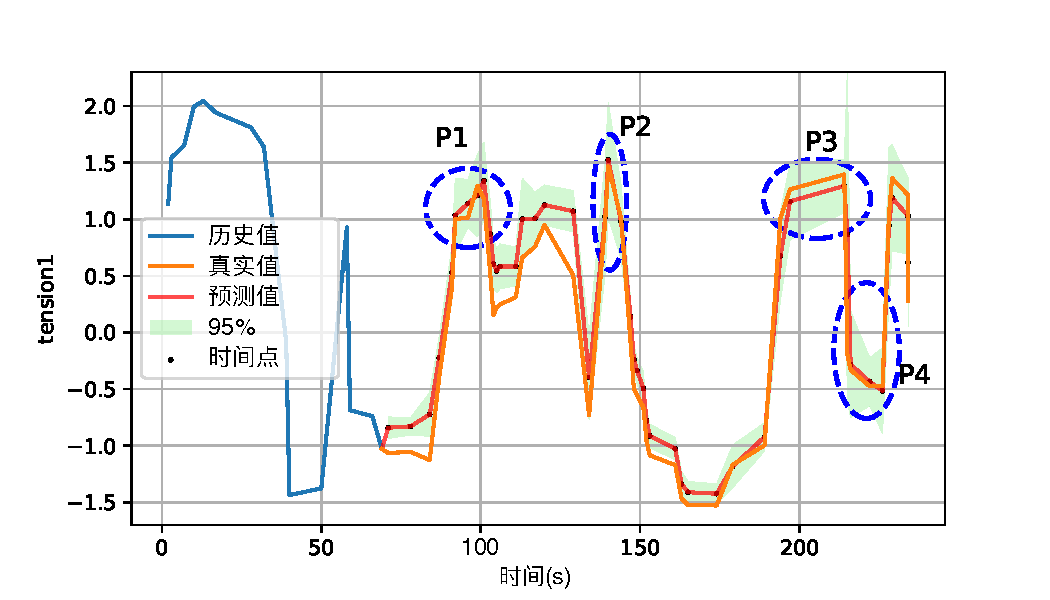
\includegraphics[width=1.1\linewidth,trim=12 0 0 20,clip]{figures/chapter5/oderssm-D_96_0.pdf}
%\caption{fig1}
\end{minipage}
\label{fig:5_predict_cmp_a}
}%
\subfigure[ODE-RSSM(RRSE=0.3080)]{
\begin{minipage}[t]{0.49\linewidth}
\centering
% \hspace{-22pt}
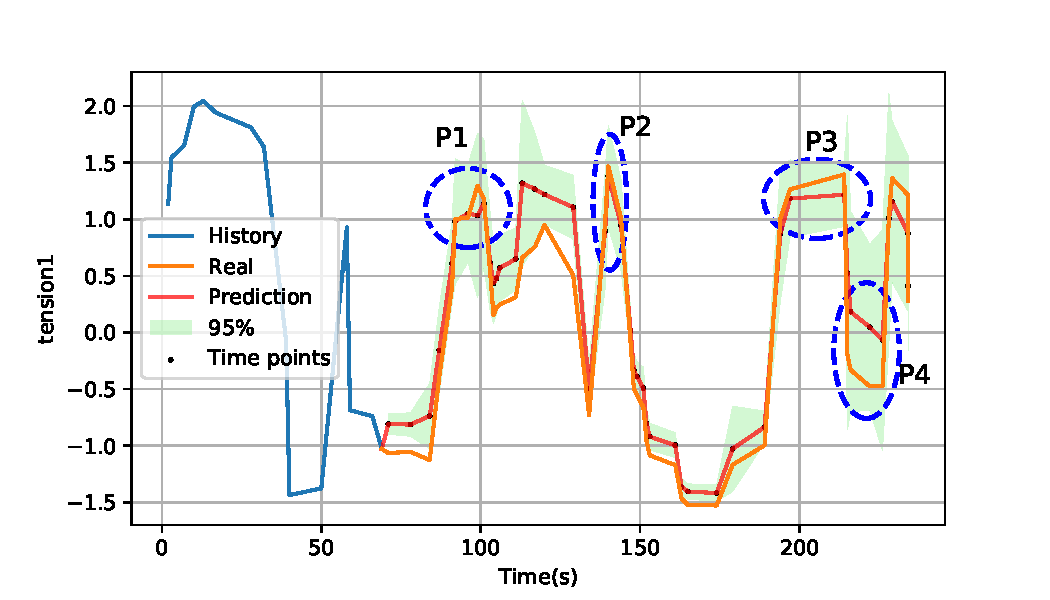
\includegraphics[width=1.1\linewidth,trim=12 0 0 20,clip]{figures/chapter5/oderssm_96_0.pdf}
%\caption{fig1}
\end{minipage}
\label{fig:5_predict_cmp_b}
}%

\subfigure[RSSM-O(RRSE=0.3345)]{
\begin{minipage}[t]{0.49\linewidth}
\centering
% \hspace{-22pt}
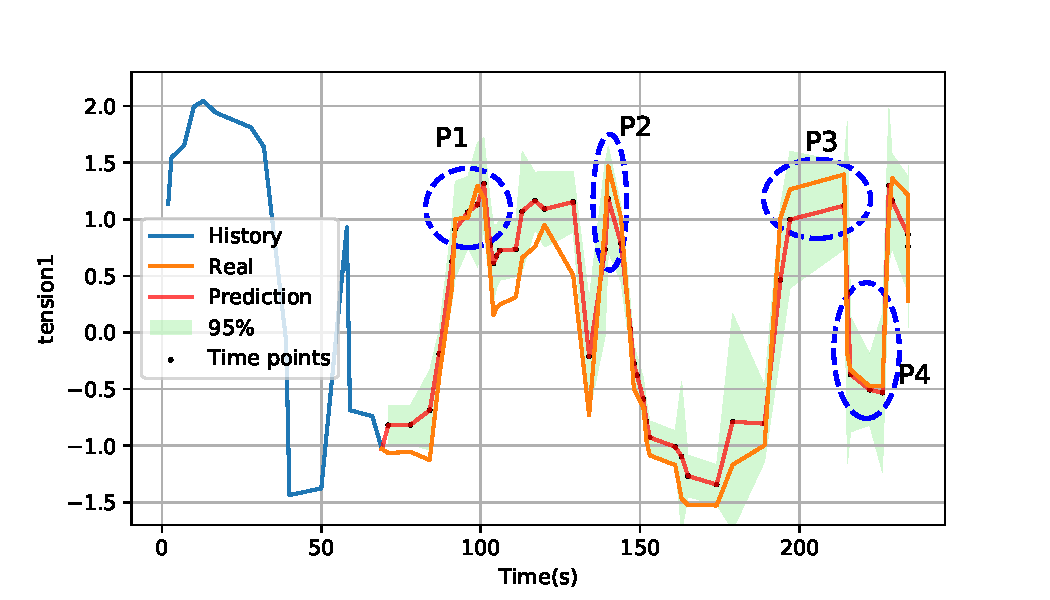
\includegraphics[width=1.1\linewidth,trim=12 0 0 20,clip]{figures/chapter5/rssm-D_96_0.pdf}
%\caption{fig1}
\end{minipage}
\label{fig:5_predict_cmp_c}
}%
\subfigure[RSSM(RRSE=0.3926)]{
\begin{minipage}[t]{0.49\linewidth}
\centering
% \hspace{-22pt}
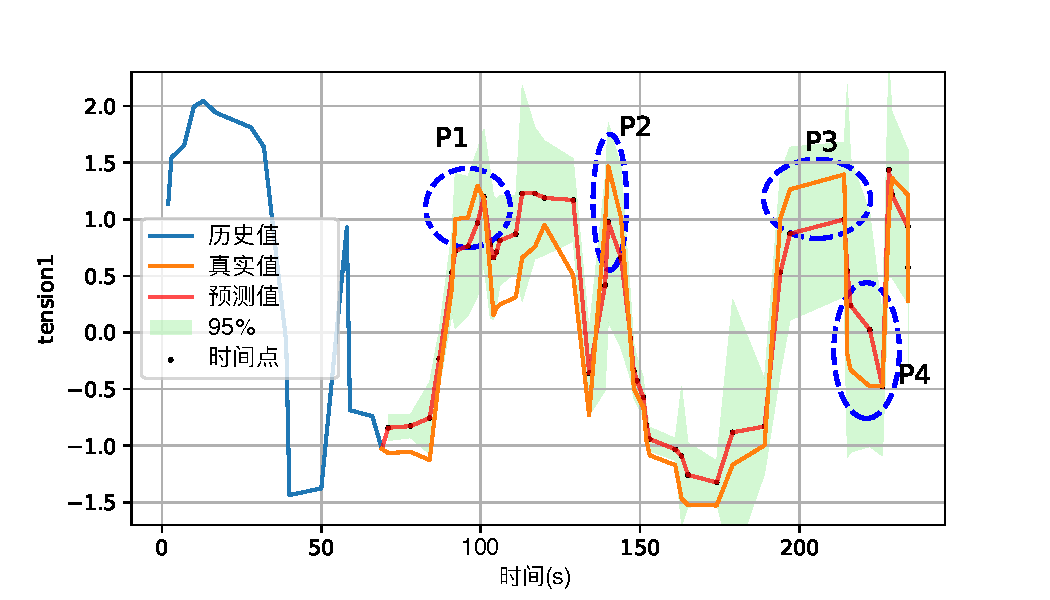
\includegraphics[width=1.1\linewidth,trim=12 0 0 20,clip]{figures/chapter5/rssm_96_0.pdf}
%\caption{fig1}
\end{minipage}
\label{fig:5_predict_cmp_d}
}%
\centering
\caption{引入微分方程网络及多步隐空间超调的效果分析}
\label{fig:5_predict_cmp}
%\vspace*{-0.4cm}
\end{figure*}
% In Figure.~\ref{fig:5_predict_cmp}, the interval between time points in position P3 is larger than the others. 
% We observe that the ODE-RSSM performs well in such sparse positions. 
% In Figure.~\ref{fig:5_predict_cmp}, We find that the ODE-RSSM significantly outperforms the discrete-time RSSM at P3, where the spacing between adjacent time points is relatively larger.
图~\ref{fig:5_predict_cmp}展示了ODE-RSSM模型和RSSM在工业绕组数据集上的某一预测片段。
可以发现,在P3处,ODE-RSSM的预测效果显著优于离散时间的RSSM。一种可能的解释是在P3处,相邻时间点之间的间隔相对较大。对于离散时间模型来说,模型主要依靠$u_t$中加入的时间差分特征$t_{i}-t_{i-1}$处理预测时间点非均匀的问题。
而此处由于$t_{i}-t_{i-1}$过大,偏离于训练集中时间差的分布,进而导致预测效果可能退化。对于ODE-RSSM模型,尽管大间距$t_{i}-t_{i-1}$会导致较大的信息损失,但对于ODE-RSSM模型的负面影响要小于对RSSM的影响。

% Although the large spacing $t_{i+1}-t_i$ leads to a considerable information loss, the brought negative effects on the ODE-RSSM model are smaller than the effects on RSSM. 
% It can be concluded that it is more effective to handle irregular time steps by learning the system evolution in continuous-time domain with a differential equation network, in comparison to adding the time delta as an extra input variable.
% This result is consistent with the previous opinions that ODE-Net enhances the performance of neural predictive models when the sequence is sparse in time\cite{Quaglino2019}.
这一结果与现有研究认为基于ODE-Net的时间序列模型更善于处理稀疏采样序列是吻合的\cite{Quaglino2019}。
% According to the results above, it can be concluded that it is more effective to handle irregular time steps by learning the system evolution in continuous-time domain with a differential equation network, in comparison to adding the time delta as an extra input variable.
相比于直接在输入量中添加时间的差分作为额外的输入变量,基于微分方程网络的系统辨识模型能够学习系统状态在连续时域下的演化,进而有效地处理非均匀采样数据。

% \subsection{RQ2: ODE-RSSM vs. Continuous-time deterministic models in stochastic systems}
% \subsection{相比于带有确定性状态演化的连续时间模型,ODE-RSSM建模随机系统的优势探究}
% \subsection{ODE-RSSM建模随机不确定性系统优势探究}

% Because the winding and thickening datasets are collected from the systems which are partially observed and full of stochasticity, they are more suitable for evaluating the models in identifying stochastic systems.
% As shown in Table.~\ref{tab:winding} and \ref{tab:thickening}, the ODE-RSSM model embed with stochastic components slightly outperform the two CT deterministic model, ODE-RNN and Time-Aware RNN.

在建模系统的不确定性方面,相比于CSTR数据集,Winding数据集和Thickening数据集来自于不确定性更强的输入输出系统,因此这两个数据集更适合于评价模型对于系统不确定性的表示能力。
% 用于对识别随机系统的模型进行评估。
% 如表所示。~\ref{tab:winding}和\ref{tab:thickening},嵌入随机成分的ODE-RSSM模型略优于两种CT确定性模型,ODE-RNN和时间感知RNN。
如表~\ref{tab:winding}和\ref{tab:thickening}所示,带有随机隐变量的ODE-RSSM模型略优于两种连续时间确定性隐状态模型。
说明在模型中引入的随机变量$\zt$有效表征了系统转移的不确定成分。
% In comparison to the deterministic models, an another advantage of the VAE-based model is 
% sampling and estimating the likelihood of a given sequence. 

% ODE-RSSM is essentially an extension of ODE-RNN that replaces the RNN updates with RSSM updates, which brings ODE-RSSM the ability to model stochastic processes.
ODE-RSSM本质上可以视为ODE-RNN模型的变种,它将瞬时状态更新过程由RNN替换为RSSM,从而使ODE-RSSM具有建模不确定性的能力。
但是当被识别系统的不确定性性较弱时,如CSTR数据集, 表~\ref{tab:cstr}说明此时采用ODE-RSSM的预测精度提升效果并不明显。
% When the identified system is approximate to a deterministic system, just like CSTR, the performance differences between ODE-RSSM and RSNN is minor, as shown in Table.~\ref{tab:cstr}.

% When the sampling interval is even uniform, 
% We firstly find that the state space models with stochastic components outperform the deterministic model, especially for the winding and thickening dataset.
% % Because both of the systems which two datasets collected from are incompletely observed and full of stochasticity.
% These two datasets are collected from the systems that are incompletely observed and full of stochasticity.
% % By introducing stochastic components, 
% Stochastic model are usually more effective for modeling such complicated stochastic systems.
% For the models in continuous-time domain, we find the stochastic components affect the accuracies of CT models in a similar way to discrete-time models.
% ODE-RSSM outperforms the other continuous-time model, ODE-RNN and Time-Aware RNN, because of embedding stochastic transitions.

% For unevenly sampled data, the ODE-RSSM model outperforms the others 
% \subsection{RQ3: Studying the effectiveness of latent overshooting }
\subsection{隐空间超调对于模型长期预测性能的影响性探究}
% In this section, we made an ablation study to verify that does introducing latent overshooting in RSSM and ODE-RSSM make improvements in prediction accuracies.
% In this section, we made an ablation study to verify the meaning of introducing latent overshooting in RSSM and ODE-RSSM.
本通过消融实验验证了在RSSM和ODE-RSSM中引入隐空间超调对于模型多步预测的改善效果。
% The results in Table.~\ref{tab:} show that introducing latent overshooting in training phases is considerablly beneficial to improve the open-loop prediction.
从表\ref{tab:cstr}至\ref{tab:thickening}可以看出,训练阶段添加隐空间超调能够有效改善模型的开环预测精度,且由于浓密机数据集存在更明显的系统时延与不确定性,改善程度更加明显。
% The improvement is more marked in the paste thickening dataset because of more obvious system delay and uncertainy.

% In Figure.~\ref{fig:5_predict_cmp}, we mark the positions P1 and P4 where the models trained by latent overshooting (a and c) outperform the ones without being trained by latent overshooting(b and d).
% 在图~\ref{fig:5_predict_cmp}中,
对比图~\ref{fig:5_predict_cmp}\subref{fig:5_predict_cmp_a}和图~\ref{fig:5_predict_cmp}\subref{fig:5_predict_cmp_c}可以发现经过隐空间超调训练过的模型在P1和P4位置的预测表现优于图~\ref{fig:5_predict_cmp}\subref{fig:5_predict_cmp_b}和图~\ref{fig:5_predict_cmp}\subref{fig:5_predict_cmp_d}中优化单步证据下限的模型。
% The reason for the improvement is that the sampling points in the two positions are intensive and the models trained with the latent overshooting technique utilize the adjacent multi-step inputs more effectively.
一种可能的解释是这两个位置的采样点较为密集,利用隐空间超调技术训练过的模型能更有效地利用相邻区域的多步输入。

% Both the tabular results and graphical illustrations demonstrate that training the generative model with multi-step KL-term improves the open-loop predictions, especially for the systems with long time delay and partially observed space .
从上述的预测指标和图形展示结果可以看出,通过优化多步KL散度项训练的生成模型可以有效改善模型的开环预测能力,特别是对于具有长时延的部分可观测系统,优化效果更加明显。
% However, the NLL of both models trained with latent overshooting are higher than the ones without latent overshooting.
% When the latent overshooting is employed, the NLL of both RSSM-O and ODERSSM-O shown are measured with setting $D=1$, which only consider the KL-divergence in single-step.
% We find the NLL in both RSSM and ODERSSM increases sharply when the latent overshooting is employed, 
% It could be explained in two aspects.
% On the one hand, when the model is trained with $D>1$, the KL-divergence in multi-steps are minimized for maximizing ELBO, which deviates from optimizing KL-divergence in single-step.
% On the other hand, in order to maximize ELBO, the encoder have to balance the KL-divergence with the reconstruction loss.
% For every inferred posterior distribution on the given sequence, the KL-divergence is measured with multiple predictive distributions when $D$ is larger than 1.
% Latent overshooting is equivalent to impose a stronger prior regularization on encoder which sacrifices the reconstruction accuracy.
% As the core topic of this paper is system identification instead of encoding and estimating log-likelihood, we are more concerned about the prediction error than likelihood.


% \subsection{RQ4: Studying the generalization ability of ODE-RSSM in varying sampling intervals}
\subsection{ODE-RSSM模型在不同采样间隔分布下的泛化能力探究}
% In this part, We conduct an experiment to study does the model trained with unevenly sampling dataset generalize to the prediction tasks, the sampling intervals of which are distinct with the ones in training dataset.
% 在本节中,我们通过实验探究使用非均匀采样数据集训练的ODE-RSSM模型是否对于任意采样间隔分布具有泛化能力,进而推广到与训练数据采样间隔分布不同的预测任务上。
本节将探究使用非均匀采样数据集训练的ODE-RSSM模型是否对于不同采样间隔分布具有泛化能力。
% ,进而推广到与训练数据采样间隔分布不同的预测任务上。
首先,本节采用工业绕组数据集(随机抽样比分别设置为0.25和0.5,非均匀采样)分别训练ODE-RSSM和RSSM模型。
% We first train the ODE-RSSM and RSSM models given the winding dataset where the random sampling ratio is set to 0.25 and 0.5 respectively.
为便于后文描述,将训练得到的四个模型命名为ODE-RSSM(25\%) ODE-RSSM(50\%), RSSM(25\%)和RSSM(50\%)。
% For simplicity, the trained four models are named as ODE-RSSM(25\%) ODE-RSSM(50\%), RSSM(25\%) and RSSM(50\%).
括号内的百分比表示训练数据集的下采样百分比。
% The percentages in parentheses represent the sampling ratio of training dataset.
% Next, we evaluate the four trained models with setting the sampling ratio as 0.25, 0.5, and 1.0.
% Next, we employ the winding dataset with the downsampling ratio, 0.25, 0.5, and 1.0, to evaluate the four trained models.
% Next, we change the downsampling ratio to 0.25, 0.5, and 1.0
% Next, we evaluate the four trained models with the downsampling ratio as 0.25, 0.5, and 1.0 respectively.
接下来,分别采用下采样比例为25\%、50\%和100\%三种情况的数据集对四个模型进行评估。
% All of the datasets in training and evaluation are unevenly sampled.
所有的训练集和测试集均为非均匀采样,
% The results on all sampling ratios are shown in Table.~\cite{tab:changing_sampling_ratio} and the differences between the prediction errors on evaluation sampling ratio and the sampling ratio of training are also recorded.
% The evaluation results on all sampling ratios are shown in Table.~\ref{tab:changing_sampling_ratio}
评估结果如表~\ref{tab:changing_sampling_ratio}所示。
% We also record the rise or the decline of the prediction error in the table corresponding to the sampling ratio of evaluation is different from the ratio in training.
% 另外,相比于测试集与训练集下采样比率相等时的测试评估结果,表中还给出了各个下采样比率下预测误差的上升或下降情况。
表中不仅给出了不同下采样比率下的评估结果,在误差指标之后的括号中还标注了相比于训练集下采样比率,预测误差的上升或下降情况。
如ODE-RSSM(50\%)模型在25\%采样比率下的RRSE记录为0.575(0.155),其中0.155代表此时的RRSE比50\%采样比率下的RRSE(0.421)高出0.155。
% 相比于测试集与训练集下采样比率相等时的测试评估结果,表中还给出了各个下采样比率下预测误差的上升或下降情况。
% 我们改变下采样比例导致的预测误差上升
表~\ref{tab:changing_sampling_ratio}结果表明将测试集的采样率从25\%提高到50\%会使得预测误差明显下降。
% The results shown in Table.~\ref{tab:changing_sampling_ratio} demonstrate that raising the sampling ratio of the test dataset from 25\% to 50\% leads to a decline of prediction error .
% We also find that the decline of ODE-RSSM(25\%) is marked and the prediction error is even lower than the ODE-RSSM(50\%).
% We even find that ODE-RSSM(25\%) outperforms the ODE-RSSM(50\%) when the sampling ratio of the test dataset is $50\%$.
甚至当测试集的采样比率为$50\%$时,ODE-RSSM(25\%)的预测误差甚至低于ODE-RSSM(50\%)。
% For the ODE-RSSM(25\%), the model have to learn from sparse sequential data and then predict the outputs with smaller intervals with the raised the sampling ratio in test dataset
对于这样的结果,一种可能的原因是当提高测试集的下采样比例时,使用ODE-RSSM(25\%)进行预测的本质是从稀疏的序列数据中学习,然后以更小的时间间隔预测输出,这一过程等价于预测和插值的组合。
% When we raise the sampling ratio in test dataset, the ODE-RSSM(25\%) have to learn from sparse sequential data and then predict the outputs with smaller intervals, which is equal to a combinational task of prediction and interpolation.
% As the previous studies demonstrate\cite{Yildiz2019}, sequential models based on ODENet have advantages in learning sparse data and interpolating.
根据以往的研究\cite{Yildiz2019}表明,基于ODE-Net的序列模型在稀疏序列数据学习和序列内插方面具有明显优势。
% Previous studies demonstrate that sequential models based on ODE-Net have advantages in learning sparse sequential data and interpolating\cite{Yildiz2019}.
% An another reason why ODE-RSSM(25\%) outperforms ODE-RSSM(50\%) when the sampling ratio equals to 25\% is that low sampling ratio reduces the noisy interferences in training dataset, which reduces the variance error of the learned model to avoid overfitting.
% An another reason for the better performance of ODE-RSSM(25\%) compared with ODE-RSSM(50\%) when the sampling ratio is 25\% is that low sampling ratio reduces the noisy interference in training dataset, which reduces the variance error of the learned model to avoid overfitting.
ODE-RSSM(25\%)比ODE-RSSM(50\%)性能更好的另一个原因是低采样率减少了训练数据集中的噪声干扰,从而减少了模型的方差,有效避免过拟合。
这一发现对于深度系统辨识的应用研究具有指导意义,合理地对训练数据进行下采样,可以更好地提升模型的泛化能力。

% When the sampling ratio in test dataset is lower than the ratio in training dataset, for instance, evaluating ODE-RSSM(50\%) and RSSM(50\%) with 25\% sampling ratio, the prediction error increases obviously and the increments of both ODE-RSSM(50\%) and RSSM(50\%) are closed to each other. 
当测试集的下采样比例低于训练数据集的下采样比时,例如用25\%采样比的测试集评估ODE-RSSM(50\%)和RSSM(50\%),此时预测误差明显增加,且ODE-RSSM(50\%)和RSSM(50\%)的误差增量是接近的。
由于低采样比会增加相邻采样时刻之间的整体长度,因此测试时求解ODE-Net的积分范围会超过训练集中时间间隔的整体分布。
% Because reducing the sampling ratio increases the overall distance between adjacent sampling points, the time ranges for solving ODE-Net greatly exceed the overall distribution of time intervals in training.
在这种外推预测下,ODE-RSSM的性能难以得到保证,但其预测精度仍然优于离散时间模型RSSM。
% The performance of ODE-RSSM is not guaranteed in such extrapolated predictions, but it is still better than discrete-time one, RSSM.

\begin{table}[htb]
\centering
\caption{
模型在测试集采样比例与训练集采样比例不同时的迁移效果评估
}
\label{tab:changing_sampling_ratio}
\resizebox{1.00\textwidth}{12mm}{
% \resizebox{\textwidth}{
\begin{tabular}{c|cccc|cccc|cccc} 
\toprule
\multirow{2}{*}{模型} & \multicolumn{4}{c|}{25\%(非均匀)}                            & \multicolumn{4}{c|}{50\%(非均匀)}                            & \multicolumn{4}{c}{100\%}                            \\
                       & \multicolumn{2}{c}{RRSE} & \multicolumn{2}{c|}{RMSE} & \multicolumn{2}{c}{RRSE} & \multicolumn{2}{c|}{RMSE} & \multicolumn{2}{c}{RRSE} & \multicolumn{2}{c}{RMSE}  \\ 
\hline
RSSM(25\%)             & 0.537 & (0)             & 0.531 & (0)              & 0.462 & (-0.075)       & 0.462 & (-0.070)        & 0.460 & (-0.077)        & 0.459 & (-0.073)        \\
RSSM(50\%)             & 0.615 & (\textbf{0.149})         & 0.607 & (\textbf{0.145})         & 0.466 & (0)             & 0.462  & (0)              & 0.460 & (-0.006)       & 0.458 & (-0.004)        \\
ODE-RSSM(25\%)         & 0.493 & (0)             & 0.488 & (0)              & 0.398 & (\textbf{-0.096})       & 0.396 & (\textbf{-0.092})        & 0.386 & (\textbf{-0.107})       & 0.384 & (\textbf{-0.104})        \\
ODE-RSSM(50\%)         & 0.575 & (0.155)        & 0.570 & (0.150)         & 0.421 & (0)             & 0.420 & (0)              & 0.380 & (-0.042)       & 0.377 & (-0.043)        \\
\bottomrule
\end{tabular}}
\end{table}


% \subsection{RQ5: Evaluating the time efficiency of the Batched ancestor sampling for estimating KL-D}
\subsection{批常微分方程并行化求解算法的时间效率探究}
% 批量常微分方程并行化求解方法
\label{sec:5_parallel_experiment}
% \subsection{Evaluating the time complexity of Parallel Reuse latent overshooting}
% In this section, we evaluate the efficiency of the proposed optimizations for accelerating the latent overshooting in training phase.
本节将对提出了的批常微分方程并行求解算法的计算效率进行评估。
% In Fig\ref{fig:6_D_time}, the time consumption of solving multi-step KL divergence are measured with linearly increased $D$ when the latent state is reused or not.
图~\ref{fig:time_cmp}\subref{fig:5_ode_time}展示了不同方法在模型训练时求解批ODE的时间消耗。
% Figure.~\ref{fig:5_ode_time} illustrates the time consumption of three methods in solving the batched ODEs.
假设训练序列的长度为$N$,其决定了批常微分方程的批大小,$I=N\times B$。
% The length of the training sequence is denoted as $N$, which determines the size of the batched ODEs, $B=N\times\text{batch size}$.
标记为“并行”的两条线代表使用式~\eqref{equ:parallel_solver}所示的积分区间变换方法并行求解多个常微分方程。
% Two of the plotted lines marked with 'Parallel' employ the proposed Interval Transformation~\eqref{equ:parallel_solver} for solving the ODEs in parallel.
% The ones marked with 'Union' solve the batched ODEs on the ordered union set of the time differences $dT=\{t_2-t_1,\cdots, t_N-t_{N-1}\}$~\cite{yildiz2021continuous,Rubanova2019}.
标记为“并集”的曲线代表构建时间差分的有序并集$dT=\{t_2-t_1,\cdots, t_{IN}-t_{IN-1}\}$~\cite{yildiz2021continuous,Rubanova2019},并按序求解有序集中所有时间点的解。
线标中的rk4和dopri5是求解ODE-Net的两个经典数值近似解算器\cite{chen2018neuralode,Yuan2022}。在本文第三章已经给出了详细介绍。

% Rk4 and dopri5 are two classical numerical approximate solvers to solve ODE-Net\cite{chen2018neuralode,Yuan2022}.
% When the solver rk4 is used, the number of calls on derivative net $f_\theta$ between any two adjacent time points is four, and the number of dopri5 becomes adaptive to ensure that the error of solutions is restricted in a given tolerance.
% rk4作为固定阶常微分方程求解器,两相邻时间点之间对导数$f_\theta$的调用次数为固定值4。
% 与之相对地,dopri5为自适应求解器,其访问导数网络的次数是自适应的,以确保解的误差在给定的误差限范围内。

% We first find that the time consumption of two methods marked with 'Union' increases linearly with the length $N$.
从图~\ref{fig:time_cmp}\subref{fig:5_ode_time}可以看出,标有“并集”的求解方法的时间消耗随长度$N$线性增加。
% In particular, the solution 'Union+rk4' consumes much more time than the solution 'Union+dopri5'.
特别地,“并集+rk4”的求解方法比“并集+dopri5”的求解方法消耗了更多的计算时间。
其原因在于当有序并集$dT$足够大时,相邻元素之间的距离特别小。
当采用自适应的dopri5常微分方程求解器时,相邻时间点之间导数的访问次数小于4次即可满足误差限要求,因此总的ODE-Net访问次数少于使用rk4求解器的访问次数。
% For the ordered union set, the distance between adjacent elements is especially small.
% When the adaptive dopri5 ODE solver is employed, the average number of the calls on ODE-Net between adjacent time points is smaller than the number by using rk4 solver.

% In comparison to solve the ODEs on the union set of time differences, the two solutions marked with 'Parallel' are more efficient.
相比于在时间点并集上求解ODE方程的解,标记为“并行”的两种求解方法效率更高。
% For the 'Parallel' solution with the dopri5 solver, the model have to guarantee the constraint of the error within a given tolerance.
% Therefore, this results in requiring more time to call the ODE-Net with the increase of batch size and sequence length $N$.
% For the parallel solution with the rk4 solver, the number of calls on ODE-Net is only four and the time consumption is irrelevant to sequence length $N$.
% The result marked with an orange line in Fig\ref{fig:5_ode_time} illustrates that the time consumption is approximately constant which is significantly less than the other three.
对于求解器组合'并行+dopri5',由于求解过程必须满足给定的误差约束,因此随着$N*B$的增加,自适应求解器评估ODE-Net的次数与时间也随之增加。
% For the choice 'Parallel+dopri5', the model has to guarantee the constraint from the given tolerances and it results in requiring more time to evaluate the ODE-Nets with the increase of length $N$.
% Therefore, it still present a linear growth of time consumption with $N$.
% For the parallel solution with the rk4 solver, in theoretically, there are only four times evaluations on ODE-Net in theoretically and the solving time is irrelevant to sequence length $N$.
% For the 'Parallel+rk4', the number of evaluations is only four and the time consumption is irrelevant to the sequence length $N$ and batch size $B$, which provides a solution for solving batched ODEs with approximate constant time complexity.
对于组合“并行+rk4”,相邻时间点之间的网络访问次数仅为4,其耗时与序列长度$N$和批大小$I$无关,该方法提供了一种求解批常微分方程的常数时间复杂度的解决方案。
% The approximate constant time complexity is significantly less than the others.
% In most cases, the sequence length $N$ is large, we therefore tend to employ the combination of reparameterization method and RK4 in training stage.

% On the assumption of infinite GPU memory and taking full advantage of CUDA parallelization, the actual time consumption of estimating the multi-step ELBO for training is approximate to $\mathcal{O}(N+D)$, where the time consumption of sequential posterior inference is $\mathcal{O}(N)$ and the time of estimating KL-D is $\mathcal{O}(D)$.
% Fig.~\ref{fig:6_D_time} illustrates the time consumption of solving multi-step KL divergence when the distance $D$ increases linearly.
图~\ref{fig:time_cmp}\subref{fig:6_D_time}说明了当距离$D$线性增加时,解多步KL散度的时间消耗。
% The blue line represents the sampled states are reused in estimating KL-D, corresponding to the Eq.~\eqref{equ:reuse}.
蓝线表示如式~\eqref{equ:reuse}所示在估计KL-D中重用采样出的隐状态。
如前文理论分析,通过重复使用中间采样潜伏状态,时间消耗讲随$D$近似线性增加。
相比之下,式~\eqref{equ:kld}所示的原始求解多步KL散度的方法所需时间是$D$的平方量级,如橙色线标记。
% When the sampled states are reused in estimating KL-D, corresponding to the Eq.~\eqref{equ:reuse}, the time consumption is mark
% As the previous theoretical analysis, reusing the intermediate sampled latent states makes the time consumption increase roughly linearly with $D$.
% In contrast, the required time of the original method~\eqref{equ:kld}, marked as an orange line, is quadratic with $D$.
% The \textcolor{orange}{orange} line represents the original method~\eqref{equ:kld} for estimating the KL-D.
% Otherwise, the required time for making multi-step predictions repeatedly is quadratic with $D$.
% For most cases, larger $D$ generally improves the performances for multi-step predictions. 
% The proposed improvement of latent overshooting reduces the training time significantly by optimizing the time complexity of estimating KL-D, in comparison to the original method.
在大多数情况下,较大的$D$通常会提高多步预测的效果。
与原方法相比,该方法通过优化KL-D估计的时间复杂度,能够显著减少$D$较大时的训练时间。

通过结合批常微方程的并行计算方法以及重用采样隐状态技巧,在拥有充足的GPU显存且充分利用CUDA并行能力的情况下,估计多步证据下限的实际时间消耗近似于$\mathcal{O}(N+D)$,其中用于后验近似推理的复杂度为$\mathcal{O}(N)$ ,估计KL-D的复杂度$\mathcal{O}(D)$。
相比于直接估计KL-D进行训练时的计算复杂度$\mathcal{O}(N+N*D^2)$
,本章提出的两个计算效率改进方法是相当可观的。

\begin{figure}[ht]
\subfigure[重参数化ODE求解器评估]{
\begin{minipage}[t]{0.49\linewidth}
\centering
% \hspace{-22pt}
% 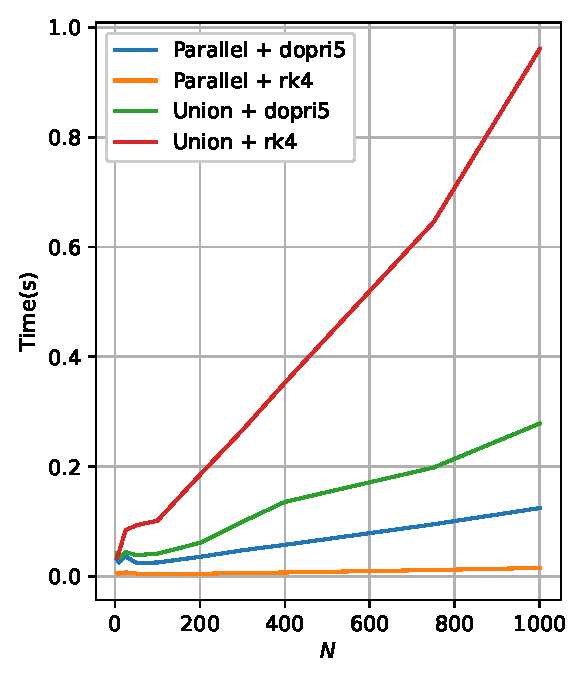
\includegraphics[width=1\linewidth,trim=0 0 0 0,clip]{figures/chapter5/ode_time.eps}
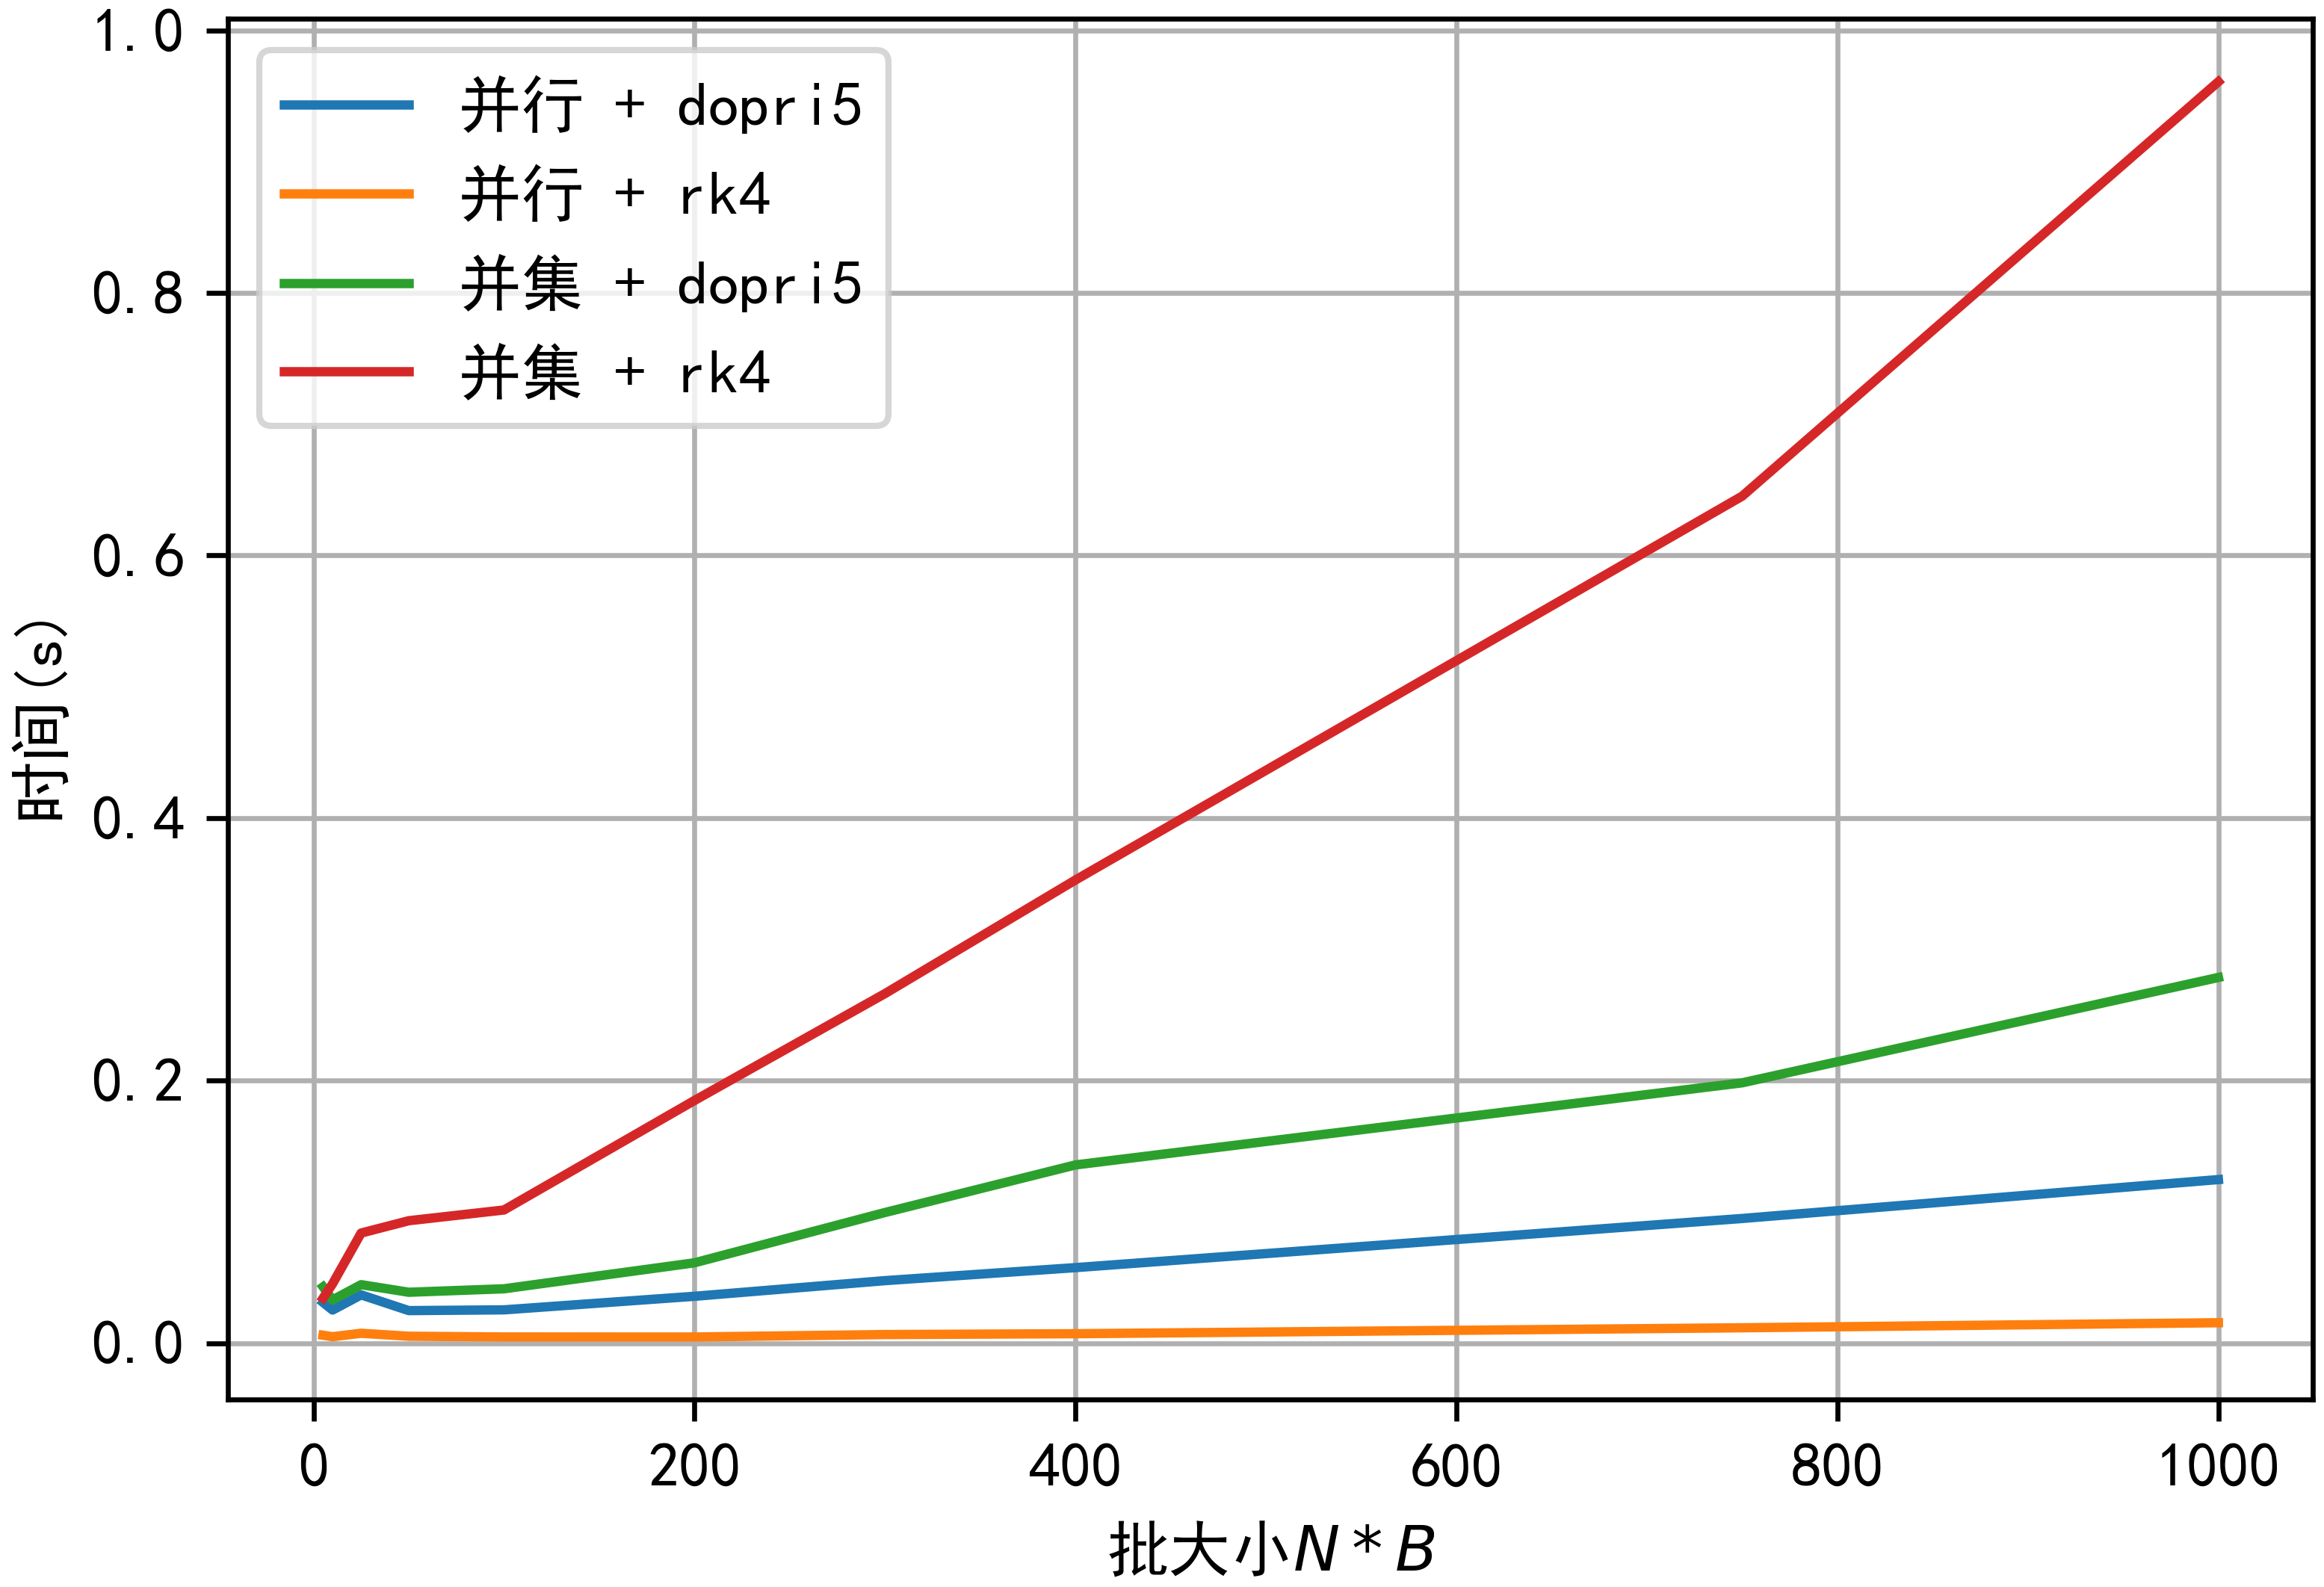
\includegraphics[width=\linewidth]{figures/chapter5/ode_time.png}
%\caption{fig1}
\end{minipage}
\label{fig:5_ode_time}
}%
\subfigure[重用采样隐状态评估]{
\begin{minipage}[t]{0.49\linewidth}
\centering
% \hspace{-22pt}
% 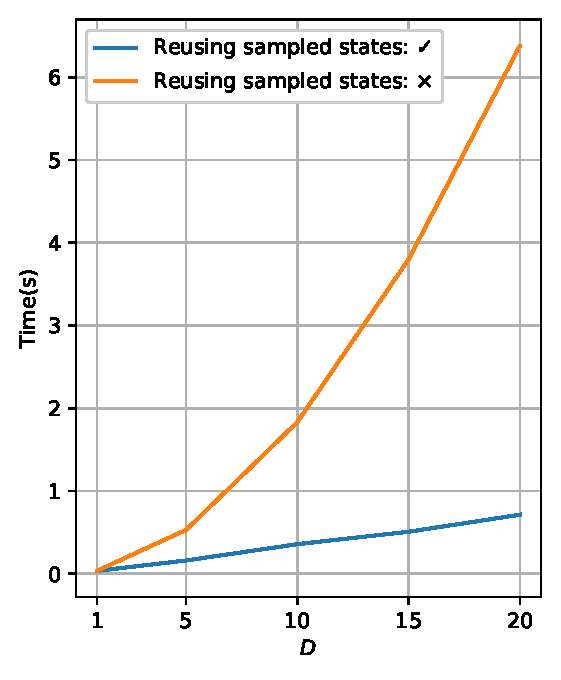
\includegraphics[width=1\linewidth,trim=0 0 0 0,clip]{figures/chapter5/D_time.eps}
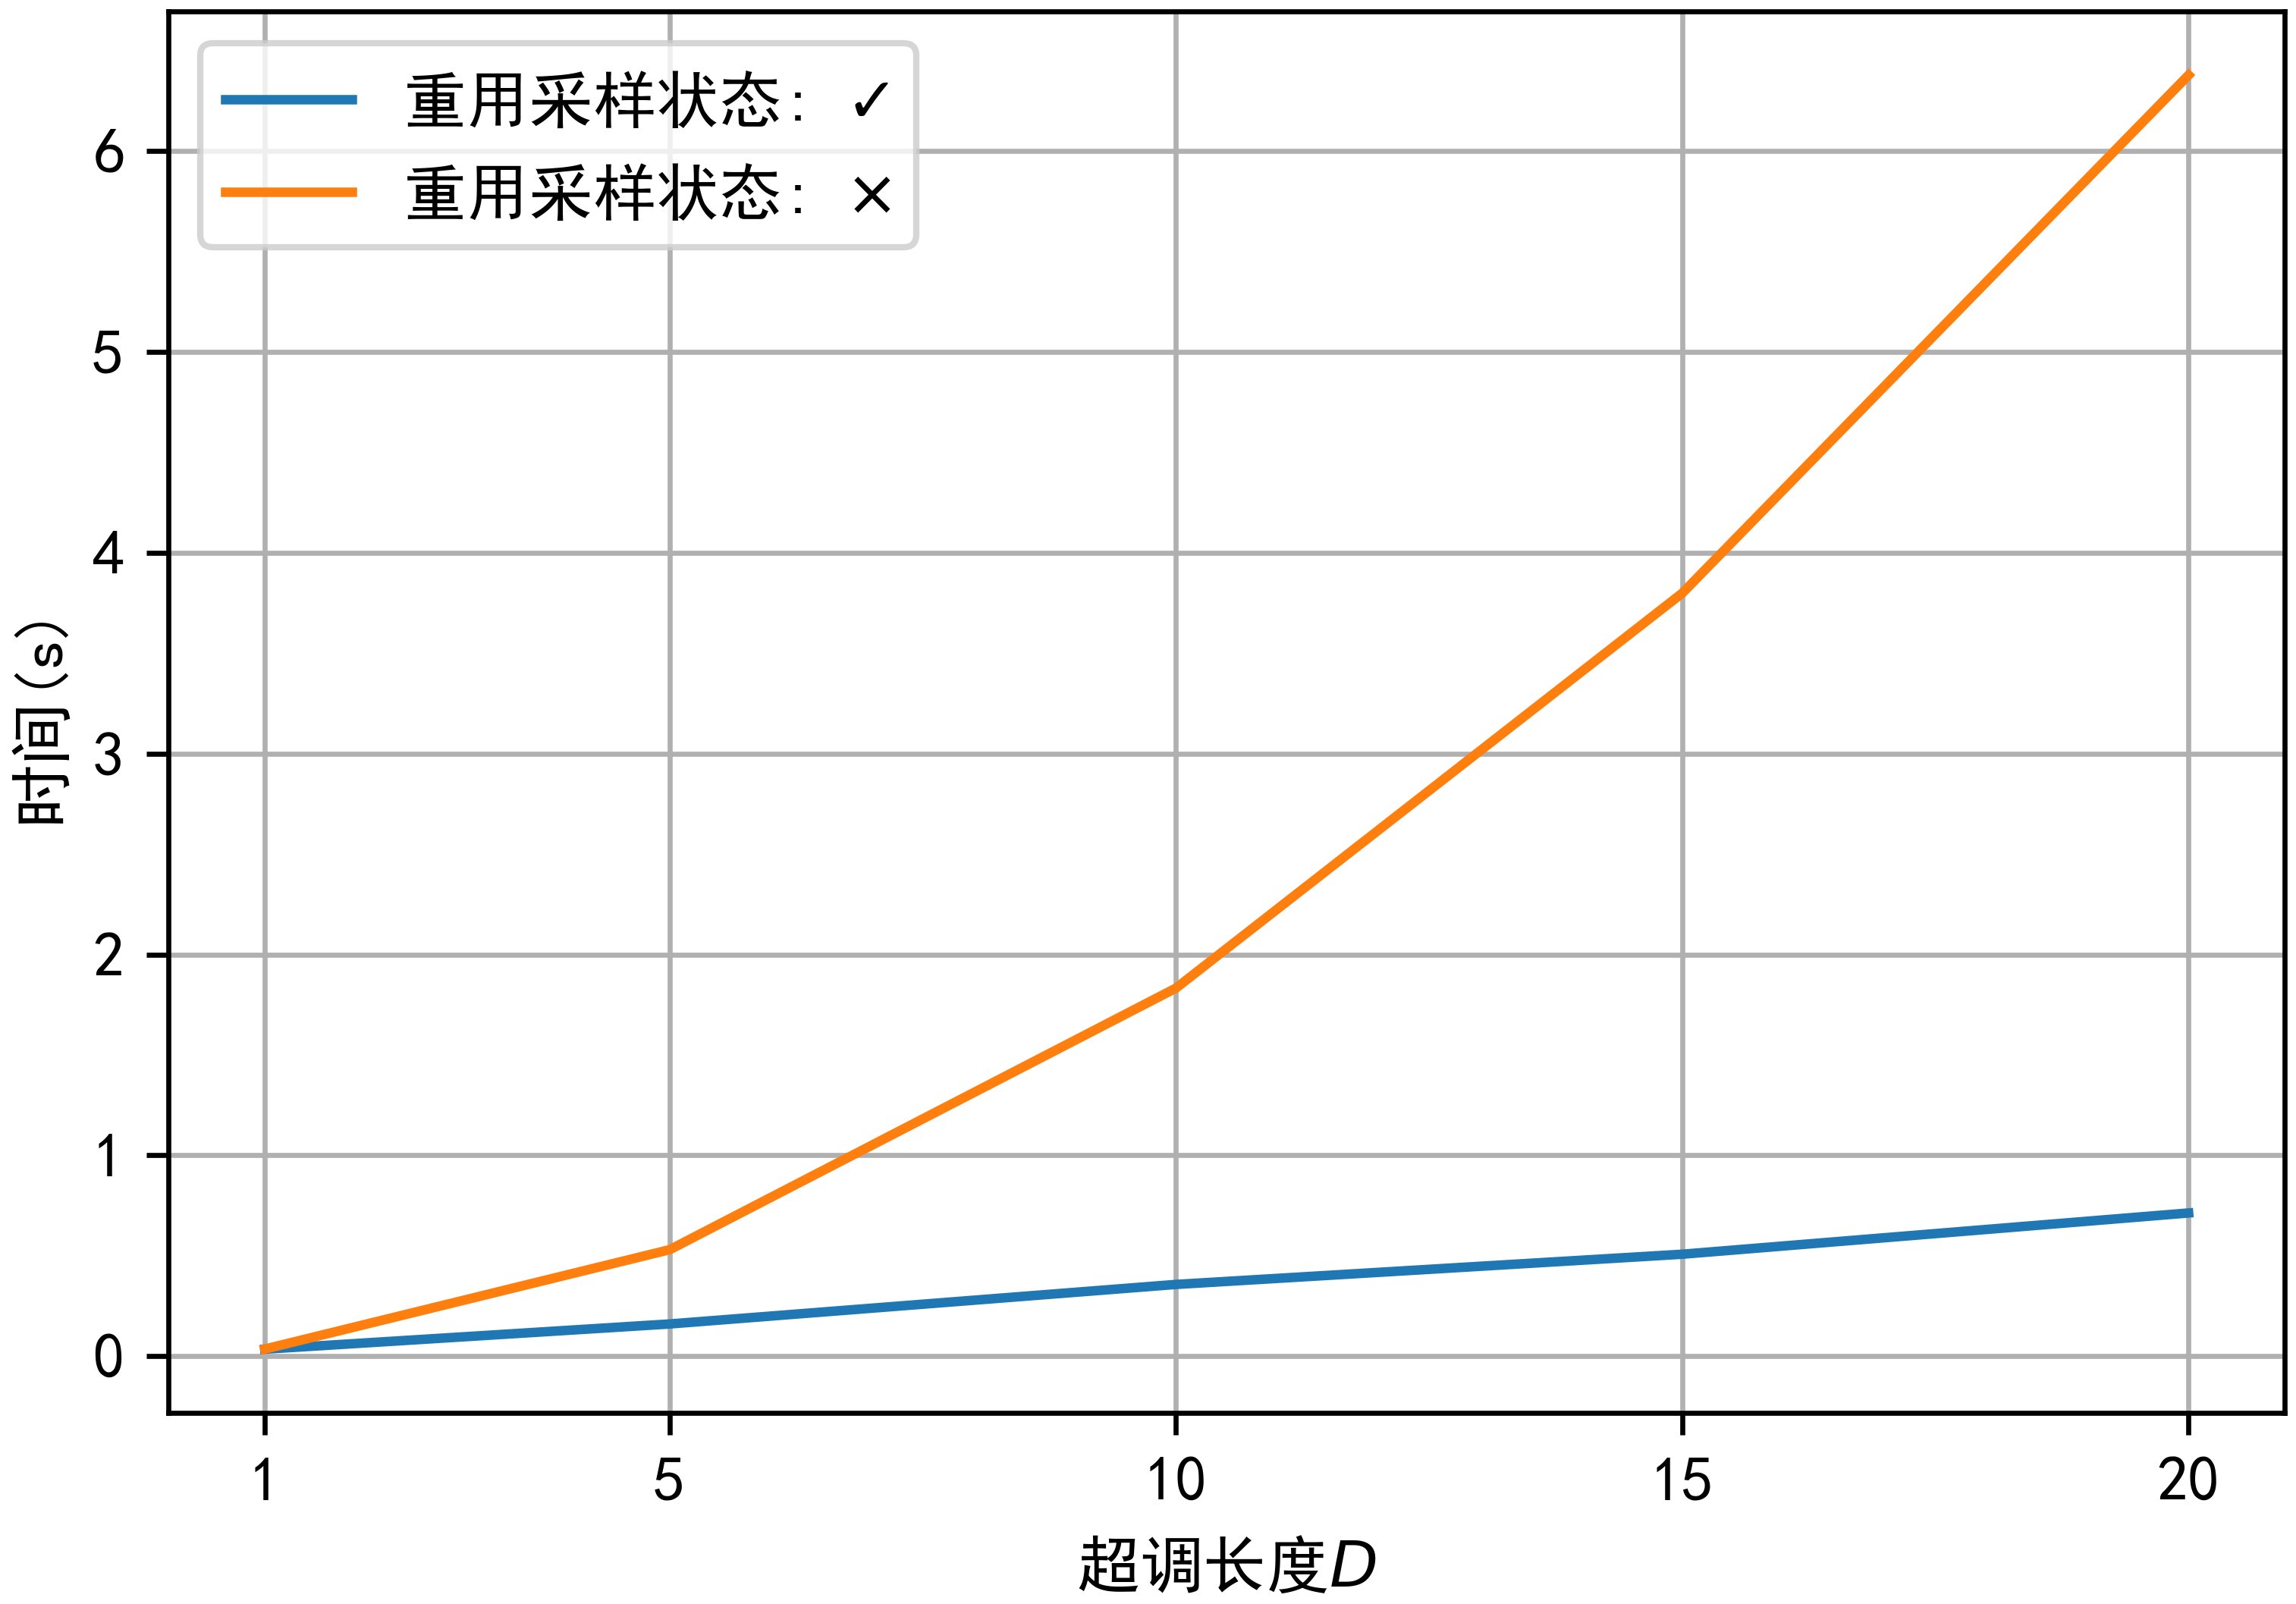
\includegraphics[width=\linewidth]{figures/chapter5/D_time.png}
%\caption{fig1}
\end{minipage}
\label{fig:6_D_time}
}%
\centering
\caption{时间复杂度改善效果评估}
\label{fig:time_cmp}
\end{figure}







% \IEEEPARstart{T}{his} demo file is intended to serve as a ``starter file''
% for IEEE journal papers produced under \LaTeX\ using
% IEEEtran.cls version 1.8a and later.
% % You must have at least 2 lines in the paragraph with the drop letter
% % (should never be an issue)
% I wish you the best of success.

% \hfill mds

% \hfill September 17, 2014

% \subsection{Subsection Heading Here}
% Subsection text here.

% % needed in second column of first page if using \IEEEpubid
% %\IEEEpubidadjcol

% \subsubsection{Subsubsection Heading Here}
% Subsubsection text here.


% An example of a floating figure using the graphicx package.
% Note that \label must occur AFTER (or within) \caption.
% For figures, \caption should occur after the \includegraphics.
% Note that IEEEtran v1.7 and later has special internal code that
% is designed to preserve the operation of \label within \caption
% even when the captionsoff option is in effect. However, because
% of issues like this, it may be the safest practice to put all your
% \label just after \caption rather than within \caption{}.
%
% Reminder: the "draftcls" or "draftclsnofoot", not "draft", class
% option should be used if it is desired that the figures are to be
% displayed while in draft mode.
%
%\begin{figure}[!t]
%\centering
%\includegraphics[width=2.5in]{myfigure}
% where an .eps filename suffix will be assumed under latex,
% and a .pdf suffix will be assumed for pdflatex; or what has been declared
% via \DeclareGraphicsExtensions.
%\caption{Simulation results for the network.}
%\label{fig_sim}
%\end{figure}

% Note that IEEE typically puts floats only at the top, even when this
% results in a large percentage of a column being occupied by floats.


% An example of a double column floating figure using two subfigures.
% (The subfig.sty package must be loaded for this to work.)
% The subfigure \label commands are set within each subfloat command,
% and the \label for the overall figure must come after \caption.
% \hfil is used as a separator to get equal spacing.
% Watch out that the combined width of all the subfigures on a
% line do not exceed the text width or a line break will occur.
%
%\begin{figure*}[!t]
%\centering
%\subfloat[Case I]{\includegraphics[width=2.5in]{box}%
%\label{fig_first_case}}
%\hfil
%\subfloat[Case II]{\includegraphics[width=2.5in]{box}%
%\label{fig_second_case}}
%\caption{Simulation results for the network.}
%\label{fig_sim}
%\end{figure*}
%
% Note that often IEEE papers with subfigures do not employ subfigure
% captions (using the optional argument to \subfloat[]), but instead will
% reference/describe all of them (a), (b), etc., within the main caption.
% Be aware that for subfig.sty to generate the (a), (b), etc., subfigure
% labels, the optional argument to \subfloat must be present. If a
% subcaption is not desired, just leave its contents blank,
% e.g., \subfloat[].


% An example of a floating table. Note that, for IEEE style tables, the
% \caption command should come BEFORE the table and, given that table
% captions serve much like titles, are usually capitalized except for words
% such as a, an, and, as, at, but, by, for, in, nor, of, on, or, the, to
% and up, which are usually not capitalized unless they are the first or
% last word of the caption. Table text will default to \footnotesize as
% IEEE normally uses this smaller font for tables.
% The \label must come after \caption as always.
%
%\begin{table}[!t]
%% increase table row spacing, adjust to taste
%\renewcommand{\arraystretch}{1.3}
% if using array.sty, it might be a good idea to tweak the value of
% \extrarowheight as needed to properly center the text within the cells
%\caption{An Example of a Table}
%\label{table_example}
%\centering
%% Some packages, such as MDW tools, offer better commands for making tables
%% than the plain LaTeX2e tabular which is used here.
%\begin{tabular}{|c||c|}
%\hline
%One & Two\\
%\hline
%Three & Four\\
%\hline
%\end{tabular}
%\end{table}


% Note that the IEEE does not put floats in the very first column
% - or typically anywhere on the first page for that matter. Also,
% in-text middle ("here") positioning is typically not used, but it
% is allowed and encouraged for Computer Society conferences (but
% not Computer Society journals). Most IEEE journals/conferences use
% top floats exclusively.
% Note that, LaTeX2e, unlike IEEE journals/conferences, places
% footnotes above bottom floats. This can be corrected via the
% \fnbelowfloat command of the stfloats package.

% \begin{center} {\centering \vbox{\centerline{\psfig{width=0.45\textwidth,figure=1.eps}}
% \vskip2mm }} \end{center} 

% \section{讨论}
% \label{sec:discussion}
% % The ODE-RSSM model encodes the evenly spaced streaming data to a continuous-time hidden state in latent space.
% ODE-RSSM模型能够对不均匀流式序列数据进行编码,并在隐空间中生成连续时间的隐状态。
% % When the new monitored system inputs and outputs are fed, the GRU module updates the deterministic hidden state and infer new stochastic latent state.
% % Otherwise, the ODE-Net predicts the evolution the $\b{h}_t$ and indirectly determines the distribution of $\b{z}_t$.
% 在同时给定新的输入输出数据时,ODE-RSSM采用GRU模块更新确定性隐状态,同时推理随机的隐变量,以此起到序列在线编码的作用。在仅有输入点时,模型能够使用ODE-Net预测$\b{h}_t$的变化并以此估计随机变量$\b{z}_t$的先验分布。
% % ODE-RSSM具备的在线编码、在线预测能力使得该模型在除系统预测以外的潜在应用。
% ODE-RSSM具备的在线编码、在线预测能力能够有效应用于除系统预测以外的问题及场景中。
% % On the basis of such property, this section will discuss the available applications of ODE-RSSM except for system prediction.

%  \textbf{模型预测控制}:在模型预测控制中(Model Prediction Control, MPC),ODE-RSSM可以作为优化过程所需的预测模型或仿真模型,
% 模型能够预测给定输入对系统序列输出的影响。ODE-RSSM支持状态循环更新的特性使其在处理增量数据时计算成本小,且优化序列长度范围灵活可变,在实际工业应用中具有很好的适用性。

% \textbf{异常检测:} 
% ODE-RSSM本质上为变分自编码器模型,利用其编码器和解码器模块能够估计给定序列数据的条件边缘似然。该似然能够作为监测数据是否存在异常的指标\cite{Xu2018}。


% \textbf{异步观测}
% ODE-RSSM假设所有通道的采样时间点是同步的。而在实际的工业系统中,不同传感器的数据采集是独立的,因此不同监测项的采集频率和采集时刻可能是不同的。
% 为了适用于此类异步观测数据,需要在模型中引入在线的数据连续化插值\cite{Che2018}技术。

% % \mathbf{Asynchronous observations} 
% % ODE-RSSM assumes the sampling time points of all channels are simultaneous. While different sensors may be observed at different frequencies in real industrial systems. 
% % It is worthwhile to incorporate online data imputation techniques\cite{Che2018} into the proposed framework.


% \textbf{时间演化过程中的随机性建模}:% ODE-RSSM is intrinsically a discrete-time model, which only infers the stochastic latent variables at discrete-time steps. 
% % The ODE-Net in CT domain only models the deterministic continuous-time evolution between adjacent observed time points.
% % In future, we look into complete continuous-time models with stochasticity, such as Stochastic Differential Equation Network(SDE), to model the continuous-time stochastic transitions of complicated system.

% 因为ODE-RSSM仅预测或推理出离散时间步下的随机隐变量分布,因此该模型本质上仍是一个离散时间模型。
% ODE-Net仅建模了相邻观测时间点之间确定性隐状态在连续时间域上的确定性演化,而无法建模状态演化过程中的存在随机性,如维纳过程等连续时间随机过程。
% 未来,本人将尝试引入具有随机性的连续时间模型作为ODE-NET的替代,如随机微分方程网络(Stochastic Differential Equation Neural Network SDE-Net),用于建模复杂系统中存在的连续时间随机性。

\section{本章小结}
\label{sec:5_conclusion}
% The conclusion goes here.
本章主要研究了如何利用非均匀间隔采样的序列数据识别具有不确定性的输入输出系统。
通过在标准的RSSM模型基础上进行扩展,本章提出的常微分方程-循环状态空间模型利用ODE-Net建模相邻观测时间点之间确定性状态的连续时间演化。
另外该模型作为状态空间模型,能够支持对流数据进行处理,进而有效解决工业传感器数据的在线推理和预测问题。
为了使模型能够在非均匀采样间隔下支持批量并行推理与训练,本章提出了一种批常微分方程并行求解算法,进而高效地求解多个积分区间不同的常微分方程。
在训练时,为了改进ODE-RSSM中生成模型的多步预测能力,本章在模型训练阶段引入了一种改进的高效隐空间超调技术。
相比于原始的多步KL散度计算方法,提出改进避免了重复的隐状态预测及采样,能够在更低的时间复杂度下获得多步KL散度的无偏估计。
% 通过将固定阶RK解算器替换为自适应解算器,求解时间步长错位的批处理隐态,
% 该方法实现了批量不规则采样序列隐态的并行预测,降低了估计KL散度为$\mathcal{O}(D)$的时间复杂度
% 这个技巧降低了对给定后验分布估计KL散度为$\mathcal{O}(D)$的时间复杂度。
在实验环节,本章对三个输入输出系统数据集的观测时间点进行随机下采样以评估ODE-RSSM及其他基线模型在不均匀数据采样下的预测效果。
结果表明,ODE-RSSM模型在不规则数据采样下,特别是高缺失率的情况下具有更好的预测准确性,对于强不确定性系统的建模效果优于确定性状态转移的连续时间系统辨识模型。
同时,基于多步隐空间超调训练的模型相比于采用单步变分下界训练的模型有更好的开环预测精度。
最后,通过对比不同序列长度以及批大小下的损失函数计算求解时间,证实批常微分方程并行求解算法以及改进的高效隐空间超调技术能够将直接估计多步变分下界的计算复杂度从$\mathcal{O}(N+N*D^2)$优化至$\mathcal{O}(N+D)$,显著增加模型效率。
% 估计KL-D的复杂度$\mathcal{O}(D)$。
% 相比于直接估计KL-D进行训练时的计算复杂度$\mathcal{O}(N+N*D^2)$
% 在讨论部分,本章分析了ODE-RSSM的应用领域及局限,并展望了未来可能继续深入的研究工作。
